%%% The main file. It contains definitions of basic parameters and includes all other parts.

%% Settings for single-side (simplex) printing
% Margins: left 40mm, right 25mm, top and bottom 25mm
% (but beware, LaTeX adds 1in implicitly)
\documentclass[12pt,a4paper]{report}
\setlength\textwidth{145mm}
\setlength\textheight{247mm}
\setlength\oddsidemargin{15mm}
\setlength\evensidemargin{15mm}
\setlength\topmargin{0mm}
\setlength\headsep{0mm}
\setlength\headheight{0mm}
% \openright makes the following text appear on a right-hand page
\let\openright=\clearpage

%% Settings for two-sided (duplex) printing
% \documentclass[12pt,a4paper,twoside,openright]{report}
% \setlength\textwidth{145mm}
% \setlength\textheight{247mm}
% \setlength\oddsidemargin{14.2mm}
% \setlength\evensidemargin{0mm}
% \setlength\topmargin{0mm}
% \setlength\headsep{0mm}
% \setlength\headheight{0mm}
% \let\openright=\cleardoublepage

%% Generate PDF/A-2u
\usepackage[a-2u]{pdfx}

%% Character encoding: usually latin2, cp1250 or utf8:
\usepackage[utf8]{inputenc}

%% Prefer Latin Modern fonts
\usepackage{lmodern}

%% Further useful packages (included in most LaTeX distributions)
\usepackage{amsmath}        % extensions for typesetting of math
\usepackage{amsfonts}       % math fonts
\usepackage{amsthm}         % theorems, definitions, etc.
\usepackage{bbding}         % various symbols (squares, asterisks, scissors, ...)
\usepackage{bm}             % boldface symbols (\bm)
\usepackage{graphicx}       % embedding of pictures
\usepackage{fancyvrb}       % improved verbatim environment
\usepackage[numbers]{natbib}         % citation style AUTHOR (YEAR), or AUTHOR [NUMBER]

%%% !!! Citation style is overriden to just a [NUMBER] !!!

\usepackage[nottoc]{tocbibind} % makes sure that bibliography and the lists
			    % of figures/tables are included in the table
			    % of contents
\usepackage{dcolumn}        % improved alignment of table columns
\usepackage{booktabs}       % improved horizontal lines in tables
\usepackage{paralist}       % improved enumerate and itemize
\usepackage{xcolor}         % typesetting in color

%% Path to images
\graphicspath{ {../img/} }

%%% Basic information on the thesis

% Thesis title in English (exactly as in the formal assignment)
\def\ThesisTitle{Automated Program Minimization With Preserving of Runtime Errors}

% Author of the thesis
\def\ThesisAuthor{Denis Leskovar}

% Year when the thesis is submitted
\def\YearSubmitted{2021}

% Name of the department or institute, where the work was officially assigned
% (according to the Organizational Structure of MFF UK in English,
% or a full name of a department outside MFF)
\def\Department{Department of Distributed and Dependable Systems}

% Is it a department (katedra), or an institute (ústav)?
\def\DeptType{Department}

% Thesis supervisor: name, surname and titles
\def\Supervisor{doc. RNDr. Pavel Parízek, Ph.D.}

% Supervisor's department (again according to Organizational structure of MFF)
\def\SupervisorsDepartment{Department of Distributed and Dependable Systems}

% Study programme and specialization
\def\StudyProgramme{Computer Science}
\def\StudyBranch{System Programming}

% An optional dedication: you can thank whomever you wish (your supervisor,
% consultant, a person who lent the software, etc.)
\def\Dedication{%
Dedication.
}

% Abstract (recommended length around 80-200 words; this is not a copy of your thesis assignment!)
\def\Abstract{%
Debugging large programs is a complex and time-consuming task, which has not 
been fully automated yet. 
Given a runtime error, the developer must first reproduce it. 
He then has to find the root cause of the error and create a proper bug fix. 
Automation can make this process significantly more efficient by reducing 
the amount of code the developer has to look through. 
This thesis introduces three methodologies of automatically reducing a given 
failing program into its minimal runnable subset. 
The techniques are based on existing findings in the field of debugging. 
The automatically minimized program must result in the same runtime error 
as the original program. 
The minimization focuses on optimal results in a domain of small and simple 
applications. 

The goal of this thesis is to discuss techniques that are practical for 
program reduction. 
These techniques are implemented using Clang LibTooling, a library for 
standalone Clang tools. 
The inner workings of each implementation are explained, and their limitations 
are exposed. 
The implementations are benchmarked on a set of C and C++ source files.  
Performance is measured based on the size of the generated output and 
the running time of the algorithm.
}

% 3 to 5 keywords (recommended), each enclosed in curly braces
\def\Keywords{%
{automated debugging}, {code analysis}, {syntax tree}, {statement reduction}, {clang libtooling}
}

%% The hyperref package for clickable links in PDF and also for storing
%% metadata to PDF (including the table of contents).
%% Most settings are pre-set by the pdfx package.
\hypersetup{unicode}
\hypersetup{breaklinks=true}

% Definitions of macros (see description inside)
%%% This file contains definitions of various useful macros and environments %%%
%%% Please add more macros here instead of cluttering other files with them. %%%

%%% Minor tweaks of style

% These macros employ a little dirty trick to convince LaTeX to typeset
% chapter headings sanely, without lots of empty space above them.
% Feel free to ignore.
\makeatletter
\def\@makechapterhead#1{
  {\parindent \z@ \raggedright \normalfont
   \Huge\bfseries \thechapter. #1
   \par\nobreak
   \vskip 20\p@
}}
\def\@makeschapterhead#1{
  {\parindent \z@ \raggedright \normalfont
   \Huge\bfseries #1
   \par\nobreak
   \vskip 20\p@
}}
\makeatother

% This macro defines a chapter, which is not numbered, but is included
% in the table of contents.
\def\chapwithtoc#1{
\chapter*{#1}
\addcontentsline{toc}{chapter}{#1}
}

% Draw black "slugs" whenever a line overflows, so that we can spot it easily.
\overfullrule=1mm

%%% Macros for definitions, theorems, claims, examples, ... (requires amsthm package)

\theoremstyle{plain}
\newtheorem{thm}{Theorem}
\newtheorem{lemma}[thm]{Lemma}
\newtheorem{claim}[thm]{Claim}

\theoremstyle{plain}
\newtheorem{defn}{Definition}

\theoremstyle{remark}
\newtheorem*{cor}{Corollary}
\newtheorem*{rem}{Remark}
\newtheorem*{example}{Example}

%%% An environment for proofs

\newenvironment{myproof}{
  \par\medskip\noindent
  \textit{Proof}.
}{
\newline
\rightline{$\qedsymbol$}
}

%%% An environment for typesetting of program code and input/output
%%% of programs. (Requires the fancyvrb package -- fancy verbatim.)

\DefineVerbatimEnvironment{code}{Verbatim}{fontsize=\small, frame=single}

%%% The field of all real and natural numbers
\newcommand{\R}{\mathbb{R}}
\newcommand{\N}{\mathbb{N}}

%%% Useful operators for statistics and probability
\DeclareMathOperator{\pr}{\textsf{P}}
\DeclareMathOperator{\E}{\textsf{E}\,}
\DeclareMathOperator{\var}{\textrm{var}}
\DeclareMathOperator{\sd}{\textrm{sd}}

%%% Transposition of a vector/matrix
\newcommand{\T}[1]{#1^\top}

%%% Various math goodies
\newcommand{\goto}{\rightarrow}
\newcommand{\gotop}{\stackrel{P}{\longrightarrow}}
\newcommand{\maon}[1]{o(n^{#1})}
\newcommand{\abs}[1]{\left|{#1}\right|}
\newcommand{\dint}{\int_0^\tau\!\!\int_0^\tau}
\newcommand{\isqr}[1]{\frac{1}{\sqrt{#1}}}

%%% Various table goodies
\newcommand{\pulrad}[1]{\raisebox{1.5ex}[0pt]{#1}}
\newcommand{\mc}[1]{\multicolumn{1}{c}{#1}}

%%% Coding packages for pseudocode
\usepackage{algorithm} 
\usepackage{algpseudocode} 
\usepackage{listings}
\lstset
{
	frame=tlrb,
	numbers=left,
	breaklines=true,
	breakatwhitespace=true,
}

%%% Todo notes
\usepackage{xargs}	% Use more than one optional parameter in a new commands
\usepackage[colorinlistoftodos,prependcaption,textsize=tiny]{todonotes}
\newcommandx{\unsure}[2][1=]{\todo[linecolor=red,backgroundcolor=red!25,bordercolor=red,#1]{#2}}
\newcommandx{\change}[2][1=]{\todo[linecolor=blue,backgroundcolor=blue!25,bordercolor=blue,#1]{#2}}
\newcommandx{\info}[2][1=]{\todo[linecolor=OliveGreen,backgroundcolor=OliveGreen!25,bordercolor=OliveGreen,#1]{#2}}
\newcommandx{\improvement}[2][1=]{\todo[linecolor=Plum,backgroundcolor=Plum!25,bordercolor=Plum,#1]{#2}}
\newcommandx{\thiswillnotshow}[2][1=]{\todo[disable,#1]{#2}}

% Title page and various mandatory informational pages
\begin{document}
%%% Title page of the thesis and other mandatory pages

%%% Title page of the thesis

\pagestyle{empty}
\hypersetup{pageanchor=false}
\begin{center}

\centerline{\mbox{
\includegraphics[width=166mm]{../img/logo-en.pdf}}}

\vspace{-8mm}
\vfill

{\bf\Large BACHELOR THESIS}

\vfill

{\LARGE\ThesisAuthor}

\vspace{15mm}

{\LARGE\bfseries\ThesisTitle}

\vfill

\Department

\vfill

{
\centerline{\vbox{\halign{\hbox to 0.45\hsize{\hfil #}&\hskip 0.5em\parbox[t]{0.45\hsize}{\raggedright #}\cr
Supervisor of the bachelor thesis:&\Supervisor \cr
\noalign{\vspace{2mm}}
Study programme:&\StudyProgramme \cr
\noalign{\vspace{2mm}}
Study branch:&\StudyBranch \cr
}}}}

\vfill

% Zde doplňte rok
Prague \YearSubmitted

\end{center}

\newpage

%%% Here should be a bound sheet included -- a signed copy of the "bachelor
%%% thesis assignment". This assignment is NOT a part of the electronic
%%% version of the thesis. DO NOT SCAN.

%%% A page with a solemn declaration to the bachelor thesis

\openright
\hypersetup{pageanchor=true}
\pagestyle{plain}
\pagenumbering{roman}
\vglue 0pt plus 1fill

\noindent
I declare that I carried out this bachelor thesis independently, and only with the cited
sources, literature and other professional sources. It has not been used to obtain another
or the same degree.

\medskip\noindent
I understand that my work relates to the rights and obligations under the Act No.~121/2000 Sb.,
the Copyright Act, as amended, in particular the fact that the Charles
University has the right to conclude a license agreement on the use of this
work as a school work pursuant to Section 60 subsection 1 of the Copyright~Act.

\vspace{10mm}

\hbox{\hbox to 0.5\hsize{%
In \hbox to 6em{\dotfill} date \hbox to 6em{\dotfill}
\hss}\hbox to 0.5\hsize{\dotfill\quad}}
\smallskip
\hbox{\hbox to 0.5\hsize{}\hbox to 0.5\hsize{\hfil Author's signature\hfil}}

\vspace{20mm}
\newpage

%%% Dedication

\openright

\noindent
\Dedication

\newpage

%%% Mandatory information page of the thesis

\openright

\vbox to 0.5\vsize{
\setlength\parindent{0mm}
\setlength\parskip{5mm}

Title:
\ThesisTitle

Author:
\ThesisAuthor

\DeptType:
\Department

Supervisor:
\Supervisor, \SupervisorsDepartment

Abstract:
\Abstract

Keywords:
\Keywords

\vss}

\newpage

\openright
\pagestyle{plain}
\pagenumbering{arabic}
\setcounter{page}{1}


%%% A page with automatically generated table of contents of the bachelor thesis

\tableofcontents

%%% Each chapter is kept in a separate file
\chapter*{Introduction}
\addcontentsline{toc}{chapter}{Introduction}

\change[inline]{TODO: Rewrite the~introduction to include goals.}

Automation of~routine tasks tied with software development has resulted in a~tremendous
increase in the~productivity of~software engineers. 

However, the~task of~debugging a~program
remains mostly manual chore. 
This is due to the~difficulty of~reliably encountering logic-based
runtime errors in the~code, a~task that, to this day, requires 
the developer's attention and supervision.

Let program $\mathcal{P}$ contain a~runtime error $E$ 
that consistently occurs when $\mathcal{P}$ is run 
with arguments $A$.
Since the~error $E$ is present at runtime and not compile-time,
it can be assumed that syntax wise the~code is mostly correct.
Therefore, any syntax-based error can be ruled out.
This, in turn, leaves us with a~set of~logical errors $\mathcal{E_L}$.
Those include wrongly indexed arrays and calculations that lead to either
the incorrect result or an altered control flow of~the program. 
Let $E \in \mathcal{E_L}$. As the~generality of~errors in $\mathcal{E_L}$
appears too complicated to be solved for all programming languages at once, 
it is necessary to break the~problem down for each programming language. 
This article is concerned with the~logical errors of~C and C++.
Although C is not a~subset of~C++, the~logical errors made in C can be
approached similarly to those in C++.
Both languages share mostly comparable constructs.
Finding the~cause of~a logical error in a~concrete language requires knowing
these constructs, their behavior, and their general handling.

To make finding the~cause of~an error a~systematic approach, one might try removing
unnecessary statements in the~code, thus minimizing the~program.
Let $\mathcal{P'}$ be a~minimal variant of~$\mathcal{P}$ such 
that $\mathcal{P'}$ results in the~same error $E$ as $\mathcal{P}$
when run with the~same arguments $A$.
If done carefully and correctly, $\mathcal{P'}$ represents the~smallest 
subset of~$\mathcal{P}$ regarding code
size, while preserving the~cause of~the error in that subset.
Upon manual inspection, the~developer is required to make less of~an effort to find
the cause in $\mathcal{P'}$ as opposed to $\mathcal{P}$.

The minimization of~a program can be achieved in numerous ways.
In further sections, the~article describes and compares three different approaches.
The first is based on naive statement removal and its consequences during runtime.
The second removes major chunks of~the code while
periodically testing the~generated program's correctness.
The third deploys a~sequence of~code
altering techniques, namely slicing and delta debugging.


\chapter{Automated debugging techniques}

\change[inline]{TODO: Link relevant literature from Slicing of LLVM bitcode (muni.cz) and Bobox Runtime Optimization (cuni.cz)}

Debugging can be described as the process of analyzing erroneous code to find 
the cause of those errors.
While most developers see debugging as a manual chore, there were numerous 
attempts~ at automating at least some parts of it during the last few decades. 
The rise in popularity of program analysis resulted in automated error checks 
for popular programming languages. 

While these checks mostly cover only specific 
cases~of potential bugs, such as out-of-range array indexing, they have proven 
themselves as a useful tool for the developer. In the context of this work, 
such checks provide a helping hand at a low cost when minimizing a program. 

The following sub-chapters will talk about the techniques behind such checks 
and how they deal with automated debugging.

\section{Delta debugging}

Delta debugging is an iterative approach described by Zeller in 1999. 
It does not perform any static analysis of the debugged program, as it 
is~not meant to find failures in the code. 

Delta debugging instead intends to 
minimize the debugged program's incorrect input to isolate the input's 
failure-inducing part. 
Therefore, it requires the program in question and the specific input 
and the expected output. 
In other words, Delta debugging requires a set of test cases, which attempts to 
minimize and isolate the failure-inducing input. Minimality is defined as follows.

\begin{defn}[Test case]\label{def02:1}
  Let $c_\mathcal{F}$ be a set of all changes $\delta_1,\dots,\delta_n$ 
  between a passing program run $r_\mathcal{P}$ and a failing program run
  $r_\mathcal{F}$ such that 
  \begin{align}
	r_\mathcal{F} = (\delta_1(\delta_2(\dots(\delta_n(r_\mathcal{P}))))). \nonumber 
  \end{align}
  We call a subset $c \subseteq c_\mathcal{F}$ a \emph{test case}.
\end{defn}

\begin{defn}[Global minimum]\label{def02:2}
  A test case $c \subset c_\mathcal{F}$ is called a \emph{global minimum}
  of $c_\mathcal{F}$ if $\forall c_i \subseteq c_\mathcal{F}:
  (|c_i| < |c| \implies c_i$ does not cause the program to fail.$)$
\end{defn}

Global minimum can be interpreted as the smallest set of changes able to
make the program fail.

\begin{defn}[Local minimum]\label{def02:3}
  A test case $c \subset c_\mathcal{F}$ is called a \emph{local minimum}
  of $c_\mathcal{F}$ if $\forall c_i \subseteq c:
  (c_i$ does not cause the program to fail.$)$
\end{defn}

\begin{defn}[$n$-minimality]\label{def02:4}
  A test case $c \subset c_\mathcal{F}$ is \emph{$n$-minimal}
  if $\forall c_i \subseteq c:
  (|c| - |c_i| \leq n \implies c_i$ does not cause the program to fail.$)$
\end{defn}

The minimizing Delta debugging algorithm attempts to find a 1-minimal test case.

Delta debugging seems to bet on the premise that large-scale applications are written
with automated testing in mind. On the same note, it is the recommended practice to
develop programs while at the same time dedicating resources to write tests for that
program.

The defined minimality can be used to construct the minimizing algorithm. 
However, the delta debugging algorithm can be easily and more comprehensively explained 
without the definition as well.

\begin{algorithm}
	\caption{Minimizing Delta Debugging Algorithm} 
	\begin{algorithmic}[1]
		\State $n \leftarrow 2$
		\State Split a string $S$ into $\alpha_1,\dots,\alpha_n$ of equal size.
		\State For each $\alpha_i$, calculate its complement $\beta_i$.
		\State Run tests on $\alpha_1,\dots,\alpha_n,\beta_1,\dots,\beta_n$.
		\If{all tests passed}
			\State $n \leftarrow 2*n$
			\If{$n > |\sigma|$}
				\Return the most recent failure causing substring.
			\Else
				\State goto (2).
			\EndIf
		\ElsIf{$\alpha_i failed$}
			\State $n \leftarrow 2$.
			\State $\sigma \leftarrow \alpha_i$.
			\If{$|\sigma| == 1$}
				\Return $\sigma$.
			\Else
				\State goto (2).
			\EndIf
		\Else
			\Comment $\beta_i$ failed.
			\State $\sigma \leftarrow \beta_i$.
			\State $n \leftarrow n - 1$.
			\State goto (2).
		\EndIf
	\end{algorithmic} 
\end{algorithm}

Additionally, minimizing is not the only approach Delta debugging suggests.
A more sophisticated one is isolation. Minimization can be described as removing parts
while the failure persists, which means that the output changes are only made in failing
iterations.
Isolation extends this by adding failure-inducing differences while the program passes tests.
This addition results in changes in both the passing and failing iterations.

One can quickly transform the input minimalization of Delta debugging into either source
code minimalization or error isolation at both the compile-time and runtime.
This transformation can be achieved for the compile-time by first setting the input
as the debugged program's source code. 
Second, it is required to set the expected
output to either 'compiled' or 'failed to compile'. 
Finally, the input is fed into a compiler, for example, GCC, which produces
one of the two set outputs. 

The runtime variant only differs in two points—first, changing the expected outputs. 
Second, changing the compiler to a compiler-debugger pipeline so that the source 
can be compiled and run.

\section{Static slicing}

The first introduced slicing method was static backward slicing. 
In 1984, Weiser defined a slice with respect to criterion C 
as a part of a program that potentially affects given variables in a given point. 

\begin{defn}[Static slicing criterion]\label{def02:5}
  Let $\mathcal{P}$ be a program consisting of program points 
  $P = p_1,\dots,p_n$ and variables $V = v_1,\dots,v_m$.
  Any pair $C = (p_i, V')$, such that $p_i \in P$, $V' \subseteq V$, and 
  $\forall v_i \in V': v_i$ is present in $p_i$, 
  is called a \emph{slicing criterion}.
\end{defn}

Slicing is the process of finding such a part of a program. 
Suggested approaches neglected any execution information and 
focused solely on observations made by analyzing the code.

\change[inline]{TODO: Convert the pseudocode to an easily readable
version (i.e. comparison with the non-sliced program).}

\begin{algorithm}
	\caption{Simple Branching Program} 
	\begin{algorithmic}[1]
		\State $x \leftarrow 1$
		\State $a \leftarrow$ read($a$)
		\For{$i = 1,2,\dots,C$}
			\State write($i$)
		\EndFor
		\If{$a$ mod $2 == 0$}
			\If{$a \neq 0$}
				\State $x \leftarrow -1 * x$
			\Else
				\State $x \leftarrow 0$
			\EndIf
		\Else
			\State $x \leftarrow x + 1$.
		\EndIf
		\State write($x$)
	\end{algorithmic}
\end{algorithm}

\begin{algorithm}
	\caption{Static Slice of the Simple Branching Program} 
	\begin{algorithmic}[1]
		\State $x \leftarrow 1$
		\State $a \leftarrow$ read($a$)
		\If{$a$ mod $2 == 0$}
			\If{$a \neq 0$}
				\State $x \leftarrow -1 * x$
			\Else
				\State $x \leftarrow 0$
			\EndIf
		\Else
			\State $x \leftarrow x + 1$.
		\EndIf
		\State write($x$)
	\end{algorithmic}
\end{algorithm}

Later that year, Ottenstein and Ottenstein restated the problem as a reachability
search in the program dependence graph (PDG).
PDG represents statements in the code as vertices and data and control
dependencies as oriented edges. 
Additionally, edges induce a partial ordering on the vertices. 
In order to preserve the semantics of the program, statements must be executed 
according to this ordering. 

Edges are, therefore, of two types. 
First, the control dependency edge specifies that an incoming vertex's 
execution depends on the outgoing one's execution. 
Second, the data flow dependence edge suggests that a variable appearing
in both the outgoing and incoming edge share a variable,
the value of which depends on the order of the vertices execution.

Once the PDG is built, slices can be extracted in linear time 
with respect to the number of vertices.

\change[inline]{TODO: Show how PDG is sliced, from 2.2 Slicing of LLVM bitcode (muni.cz)}

However, one can find many potential issues and obstacles when performing 
data flow analysis. 
Omitting the interprocedural slicing, as it is not relevant in this paper's
context, one is left with pointers and unstructured control flow.
While the latter is seldomly used in single-threaded modern programming, 
the same cannot be said about the former. 

Pointers require us to extend the syntactic data flow analysis 
into a pointer or points-to analysis, which should be performed first. 
It is necessary to keep track of where pointers may point to (or must point to,
in case their address is not reassigned) during the execution. 
From this knowledge, other data flow edges must be created or
changed to accommodate the fact when the outgoing vertex mayhap writes
into a memory location possibly used by the incoming vertex. 

The analogical approach is then used for control dependency analysis since 
pointers might alter control flow as well. 
This change to control flow happens, namely when functions are called using 
function pointers.

The main advantage of static slicing is that it does not require
any runtime information. 
As program execution can be expensive both time-wise and resource-wise, 
static slicing offers program comprehension at a low cost. 
Because static slicing discovers program statements that can affect 
certain variables, it can remove dead code and be used for program segmentation. 

Furthermore, static slicing is used for testing software quality, maintenance, 
and test, all of which are relevant to this project.

\section{Dynamic slicing}

While the idea of building a program slice prevails, dynamic slicing 
drastically differs from static slicing in terms of input and the way
it is processed. 

In 1988, Korel and Laski described a slicing approach that took into 
consideration information regarding a program's concrete execution. 
As opposed to static slicing, which builds a slice for any execution, 
dynamic slicing builds a slice for a given execution of a program. 
Using information available during a run of the program 
results in a typically much smaller slice.

\change[inline]{TODO: Convert the pseudocode to an easily readable
version (i.e. comparison with the non-sliced program).}

\begin{algorithm}
	\caption{Dynamic Slice of the Simple Branching Program (for $a = 2$)} 
	\begin{algorithmic}[1]
		\State $x \leftarrow 1$
		\State $a \leftarrow$ read($a$)
		\State $x \leftarrow 0$
		\State write($x$)
	\end{algorithmic}
\end{algorithm}

This decrease in size is mainly due to removing unnecessary 
branching of control statements and unexecuted statements in general. 
The slicing criterion now contains a set of the program's 
arguments in addition to the previous information. 
The location of the criterion's statement is also specified to avoid 
vagueness in the execution history. 

The criterion is therefore defined as follows.

\begin{defn}[Dynamic slicing criterion]\label{def02:5}
  Let $\mathcal{H} = (s_{x1},\dots,s_{xn})$ be an execution history of a program 
  $\mathcal{P} = (\{s_1,\dots,s_m\}, V)$, where $s_i$ denotes a statement
  and V is a set of variables $v_1,\dots,v_k$.
  Any triple $C = (h_i, V', \{a_1,\dots,a_j\})$, such that $h_i \in \mathcal{H}$,
  $V' \subseteq V$, $\forall v_i \in V': v_i$ is present in $h_i$,
  and $\{a_1,\dots,a_j\}$ is the input of the program,
  is called a \emph{slicing criterion}.
\end{defn}

Since dynamic slicing requires the user to run the program, 
it is typically used in cases where the execution with a fixed 
input happens regardless. Such cases include debugging and testing. 
For debugging, dynamic slices must reflect the subsequent restriction: 
a program and its slices must follow the same execution paths.

\section{Summary}

While the described program minimizing and debugging approaches have been 
formulated more than two decades ago, there have not been nearly enough 
successful attempts at implementing them. 

With each approach having its clear positives and negatives, 
it would be interesting to see how they handle program minimization. 
When cleverly used, a combination of these methods might 
result in a reasonably fast and inexpensive algorithm 
for the reduction of program size.
\chapter{Compilers and analysis tools}

In the~previous chapter, the~reader was introduced to a~branch of~program
ana\-ly\-sis. 
The techniques discussed above focused on both the~static and runtime
side of~program analysis. 

Regardless of~whether these approaches have been implemented, it was 
required to find a~suitable tool for source code manipulation for two reasons. 
First, any external tool output might require altering the~input source code 
based on its output. 
Second, if implementing any code reducing algorithm would have to occur, 
one would need a~sophisticated code modifying framework. 

Due to these reasons, an analysis of~compilers and tools for C and C++ was conducted. 
The goal of~the~analysis is to pick the~most practical tool available. 
Required criteria include frequent upkeep of~the~framework, 
an existing user base, and the~ability to manipulate some abstract 
representation of~the~code.

The representation boiled down to an abstract syntax tree (AST). 
AST embodies the~syntactic structure of~the~code, regardless of~the~code's language. 
A vertex of~an AST represents a~construct of~the~code while not being concrete 
with the~details of the code's programming language. 
This generality is perfect for C and C++'s chosen domain, 
as both languages only differ syntax-wise in~minor details.

Below are the~findings concerning the~most important candidates.

\section{GCC}

A well-known C and C++ compiler, the~GNU Compiler Collection \citep{gcc:online} 
is an extensive
open source project. 
As popular as GCC is, it does not provide the~features an analysis-tool-building 
developer needs. 

For the~sake of~building such tools, a~compiler front end is used. 
Due to an old design, it is difficult to work with either the~front end or 
the back end of~GCC alone. 
Besides, the~compiler implicitly makes optimizations that destroy any parallels 
between the~source code and the~AST. 
Therefore, the~AST has to be treated as an entirely different object rather than 
an abstraction of~the~code. 
Most of~the~compiler's source code representation is unintuitive and 
hard to pick up for anyone not actively contributing to GCC. 
Figure~\ref{img:gcc} showcases the~unfriendliness rather well.
Compared to figure~\ref{img:pdg}, which is an output of~a~tool built using
LLVM and Clang, GCC's mapping between the~source code and the~internal
representation does not hold up.

As far as AST manipulation is concerned, the~compiler allows the~user to dump 
the structure into a~text representation. 
However, due to the~difficulties mentioned above, it can hardly be used.

\begin{figure}[p]\centering
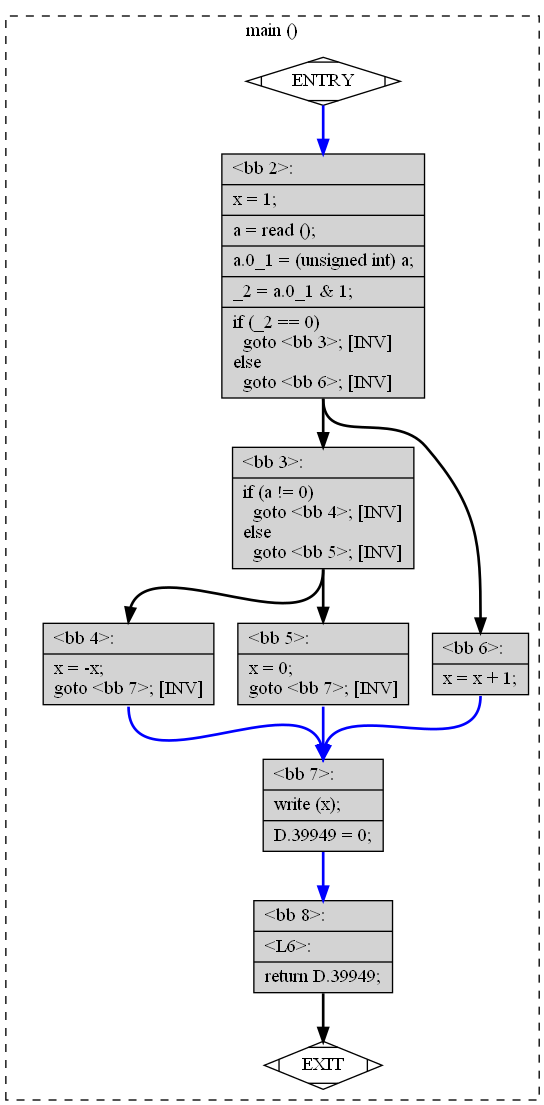
\includegraphics[scale=0.55]{gcc_ast}
\caption{GCC AST Dump. This figure showcases 
the AST representation of~\ref{lst:simpleexample}
as dumped by GCC. Note that it is not easily comprehendable.}
\label{img:gcc}
\end{figure}

These issues result in~a seldom-used variant that offers nearly 
no developer-friendly features. 
An upside is that GCC allows the~user to visualize the~AST. 
However, that is hardly a~useful feature in~the context of~this paper.

\section{Clang}

Thanks to LLVM \citep{llvm:online}, the~widespread compiler infrastructure,
the Clang project \citep{clang:online}
has provided a~compiler front end not only for C and C++ but also 
for CUDA, OpenCL, and other mainstream programming languages. 
The extend of~Clang as a~compiler front end is so vast that it covers 
both the~C++ standard and the~unofficial GNU++ dialect.

The project does not include just the~front end but also a~static analyzer 
and several code analysis tools, which are now commonly used in~IDE's as 
syntax and semantic checks. 

This description of~Clang foreshadows its friendliness to analysis tool developers. 
The fact that the~front end runs on a~common intermediate language also indicates 
that openly working with abstract code representations is supported.

There are three most notable interfaces for customizing Clang. 
Firstly, the LibClang interface allows the~users to write 
comprehend-able high-level code with limited functionality. 
On the~other hand, LibTooling gives the~user much more control 
at the~cost of~a~steep learning curve. 
Lastly, the~Plugins interface features similar difficulty 
as LibTooling with a~more specific goal. 
Plugins are used with the~Clang compiler and can be run 
as a~front-end action when called during compilation.

\section{ANTLR}

A less typical way of~extracting an AST from a~source file is by using grammar
recognition.
ANTLR \citep{antlr:online}, which stands for Another Tool for 
Language Recognition, is a~free 
parser generator that generates both a~lexer and a~parser based on 
a given grammar.
Additionally, ANTLR can also generate a~tree parser.
Tree parsers are helpful in~processing ASTs.

The tool is generally used to read data formats, process expressions 
of various query languages, and even parse source code written in complex 
programming languages.
It can be used to generate a~syntax tree and walk through it using a~visitor.
ANTLR is based on the~LL parser, which parses the~input from left to right, 
performing its leftmost derivation.

To create a~parser or a~syntax tree of~code written in a~programming language, 
ANTLR requires the complete grammar of~that language.
Some programming languages, namely C and C++, have an ambiguous syntax that 
is hard to parse based solely on its grammar.
Due to ANTLR's high popularity, many grammars have already been written 
for it.
As far as C++ is concerned, its C++14 standard's grammar is the~most recent 
one available.

Writing grammar for newer standards or creating a~custom one for both C and 
C++ would be unnecessarily burdensome for this project.
This statement holds, especially when considering other tools mentioned above.

The most recent release, ANTLR 4, added more options for grammar rules.
Most notably, it supports direct left recursion.
However, that still might not be enough to choose it over other tools.


\section{DMS}

Similar to ANTLR, the~DMS Software Reengineering Toolkit \citep{dms:online}
features a~parser generator.
The tool is proprietary software created by Semantic Designs.
Besides the~mentioned parser generator, it features an entire toolkit for 
creating custom software analysis.
This toolkit is used mainly for reliable refactoring, duplicate code 
detection, and migration of the source code's programming language.

The parser generator part takes a~grammar and produces a~parser.
This parser then constructs abstract syntax trees for provided source code.
Additionally, created ASTs can be converted back to source code using 
prettyprinters.
The parser saves additional information about provided source files, such as 
comments and formatting.
It can then recreate the~file accurately.

DMS provides a~grammar for a~large number of~programming languages, 
including C and C++.
The language support, however, is not always up-to-date.
The newest supported C++ standard is still the~older C++17.
These complicated grammars' ambiguity is avoided using a~generalized 
left-to-right parser, which performs the~rightmost derivation (GLR).
Since DMS provides refactoring ability as well, it allows for transformation 
rules in~the grammar.

Another helpful feature of~the~toolkit is control flow and data flow analysis.
Analyzing control flow and data flow, generating their graphs, and performing 
the points-to analysis (also supported by DMS) is practical when considering
static slicing (section 1.2).

It should be noted that some of~the~free, open-source tools mentioned above 
do a~better job of~being a~so-called 'software analysis toolkit' than 
DMS does.

\section{Summary}

The chapter highlighted a~spectrum of~tools, ranging from language
recognizers to compilers.

It would seem that parsing source code written in multiple programming 
languages into an abstract representation requires a~common intermediate 
language, in~which the representation is stored. 
Having an intermediate language is not always possible for several reasons, 
including licensing and old architecture. 
The compiler giant GCC seems to suffer from precisely that.
Additionally, since the~Clang project is being contributed to regularly, 
resulting in~as many as five releases per year, 
it pulls in~a more significant developer community. 

Therefore, Clang is the~favorite source code altering tool for this project. 
In the~following chapter, the~relevant parts of~the~Clang project 
will be broken down and explained.

\chapter{Clang LibTooling}\label{chap:libtooling}

The previous chapter described tools and environments that were taken
into consideration for this project. 
The utmost importance was given to the~ease of~use, availability, and 
active community. 
As the~reader might have guessed from the~summary, the~LLVM/Clang 
suite stood out as the~best candidate.

Clang is a~language front-end. With high compilation performance, 
low memory footprint, and modifiable code base, it quickly and flexibly 
converts source code to LLVM intermediate code representation. 
The front-end supports languages and frameworks such as C/C++, 
Objective C/C++, CUDA, OpenCL, OpenMP, RenderScript, and HIP. 
This support is crucial for this thesis since the~project 
aims to support both C and C++. 
The LLVM Core then handles the~optimization and IR synthesis, 
supporting a~plethora of~popular CPUs.

Clang is widely used for its warnings and error checks, both very 
helpful and outstanding compared to competing compilers. 
Furthermore, Clang offers an extensive tooling infrastructure 
through which tools such as clang-tidy were developed. 
A relatively well-documented tooling API written in~C++ helps 
programmers create their tools easily. 
However, not all developers share the~same skill set. 
Some programmers require complicated additional features, while others 
prefer an easy-to-use interface. 
The tooling API has been split into multiple libraries and frameworks,
including Plugins and LibClang.
Explaining the two mentioned libraries is necessary. 
It is essential to show their capabilities before introducing LibTooling. 
LibTooling is the tooling library ultimately chosen for this project.

\paragraph{Plugins.}

The~library intuitively called Plugins is used for plugin development.
The library is linked dynamically, resulting in~relatively small tools.
Plugins are launched at compilation and offer compilation control as well 
as access to the~AST.

More specifically, Plugins allow performing an extra custom front-end action 
during compilation.
The functionality is generally similar to that of~LibTooling, which will be 
talked about later.
However, unlike a~standalone tool, Plugins cannot do any tasks before and after 
the analysis (and compilation).
When creating a~plugin, one can choose from a~selection of~
\icode{FrontendAction} classes to inherit.
If, for example, the~plugin should work with the~AST, 
the \icode{ASTFrontendAction} can be inherited.
Doing so also allows overriding the~\icode{ParseArgs} method, in~which 
the plugin's command line handling is specified.

Due to dynamic loading, the~wanted plugin must be added to a~plugin registry 
inside the~code.
The plugin is then loaded from the~registry by specifying the~\icode{-load} 
command or \icode{-fplugin} on the~command line when running clang.
The plugin takes those arguments from the~command line that are prefixed 
by \icode{-Xclang}.

\paragraph{LibClang.}

Another framework, LibClang, offers a~simple C and Python API for quick 
tool writing. 
Unlike Plugins and LibTooling, which will be mentioned later, the~code 
base of~LibClang is stable. 
This stability implies that tools written using LibClang do not require
upkeep with every new LLVM/Clang release. 
Overall, the~framework and tools written using it are high-level and 
are easily readable.

\paragraph{LibTooling.}

The most feature woven set of~libraries is LibTooling. 
Unlike Plugins, LibTooling \citep{libtooling:online} 
allows the~developer to build standalone 
Clang tools. 
This robust framework is written in~C++ and has an active 
community of~contributors. 
One can find many manuals and tutorials online. 
However, with each contribution to LibTooling and each release of~Clang, 
there is a~chance that older tools will not support the~newer LibTooling 
API. 
That is the~reason why countless tools written using this framework do not
run in~modern environments. 
Programmers who use LibTooling cannot expect compatibility in~upcoming 
releases. 
On the~bright side, the~libraries of~LibTooling allow a~plethora of~source
code modifications, AST traversals, and access to the~compiler's internals.

The set of~features supplied by LibTooling is immense. 
The following sections describe notable features used during 
the implementation of~this project. 
The reader should get a~better idea of~how a~tool is built and what 
LibTooling offers during the~development process. 
Important concepts, such as providing the~correct input to the~tool 
in the~form of~a~compilation database, traversing the~AST, 
and modifying source code inside the~tooling environment, 
are described below. 
These concepts will be referenced further in~the text.

\section{Compilation databases}

To accurately and faithfully recreate a~compilation, tools created using 
LibTooling require a~compilation database (CD) \citep{cd:online} 
for a~given input project.

The motivation behind a~CD is simple.
If a~source file uses unusual include paths that need to be provided 
using the~\icode{-I} compiler command, it cannot be reliably compiled.
Similarly, if the~file contains macros and lacks definitions, its content 
can drastically change when the~definitions are present.
In the~latter case, definitions are provided to the~compiler 
with the~\icode{-D} command.
Such compiler commands, options, and flags are usually defined in~a build 
system.
At least, that is the~recommended practice for larger projects.
Having a~build system is similar to having a~CD.
It is clear which file is compiled with which options.

Clang expects a~CD in~the JSON format and looks for the~file specifically
named  \icode{compile\_commands.json} in~the current or parent 
directories.
The JSON file contains entries for source files.
Each entry contains a~directory, a~file name, and a~compilation command.
Multiple entries for a~single source file are also valid.
Such a~case can arise when performing repeated compilation.

As previously mentioned, having a~build system helps.
Build tools such as CMake and Ninja can be used to generate a~CD.
If the~project is not using any of~the~compatible build tools, 
the user can either make a~CD manually or use an external tool.
One such tool is Build EAR available at \url{https://github.com/rizsotto/Bear}.

Tools created using LibTooling do not always require compilation databases 
to run.
For simple projects, they can take the~\icode{-{}-} argument that separates 
the tool's arguments from the~project's compilation arguments.
One can interpret the~arguments following \icode{-{}-} as a~temporary
compilation database.

\section{Clang AST}\label{chap:ast}

The abstract syntax tree used in~the Clang front-end \citep{ast:online}
is different from the~typical AST. 
It saves and carries more data, namely context.  
For example, it contains additional information to map source 
code to nodes and capture semantics. 
This chapter describes the Clang node type hierarchy, the tree's 
representation in memory, and different ways of traversing an AST.
\subsection{Node types}

Clang AST's nodes belong to a~vast class hierarchy. 
This hierarchy contains classes that represent every supported 
source code construct.
Nodes are of~four different types: statements (\icode{Stmt}), 
declarations (\icode{Decl}), specific declaration context 
(\icode{DeclContext}), and types (\icode{Type}). 
However, in~the APIs mentioned above, the~nodes do not share
a common ancestor.

The children of~\icode{Type} represent all available types.
The goal is to give each type in~the source code a~canonical type,
i.e., a~type stripped of~any typedef names. 
Canonical types are used for type comparison, while non-canonical 
types give complete information during diagnostics. 
The \icode{Decl} hierarchy's goal is to have a~class for each 
type of~declaration or definition. 
These declarations vary, and the~children cover specific cases 
such as function, structure, and enum declarations. 
Some declarations, such as function and namespace declarations, 
capture additional data in~\icode{DeclContext}'s children. 
The final node type, \icode{Stmt}, represents a~single statement. 
It has subclasses for loops, control statements, compound statements, 
and more. 
Additionally, expressions (\icode{Expr}) also belong 
to the~\icode{Stmt} hierarchy.

Figure~\ref{dia:ast} shows a~part of~the~class hierarchy. 
The entire class diagram cannot be shown as there are over a~thousand 
different classes\footnote{The class hierarchy is shown in~Clang's
Doxygen documentation. An example of~the~Stmt hierarchy can be found
at \url{https://clang.llvm.org/doxygen/classclang_1_1Stmt.html}.}. 
The topmost node, the~root, of~a~concrete Clang AST is called the~translation
unit declaration (\icode{TranslationUnitDecl}). 
Edges between nodes are simplified, as each node stores 
a container of~its children.

\begin{figure}[ht]\centering
\begin{tikzpicture}
	\begin{class}[text width=2cm]{Stmt}{-5.5, 0}
	\end{class}

	\begin{class}[text width=2.5cm]{ValueStmt}{-5.5, -6}		
		\inherit{Stmt}
	\end{class}

	\begin{class}[text width=2cm]{Expr}{-5.5, -8}
		\inherit{ValueStmt}
	\end{class}

	\begin{class}[text width=1.75cm]{IfStmt}{-4.25, -2.75}
		\inherit{Stmt}
	\end{class}

	\begin{class}[text width=2cm]{Type}{-2, 0}
	\end{class}

	\begin{class}[text width=2.5cm]{ArrayType}{-3.5, -4.25}
		\inherit{Type}
	\end{class}

	\begin{class}[text width=3cm]{DeducedType}{-2, -6}
		\inherit{Type}
	\end{class}

	\begin{class}[text width=2.5cm]{AutoType}{-2, -8}
		\inherit{DeducedType}
	\end{class}

	\begin{class}[text width=2cm]{Decl}{1.5, 0}
	\end{class}

	\begin{class}[text width=2.5cm]{EmptyDecl}{-0.25, -2.75}
		\inherit{Decl}
	\end{class}

	\begin{class}[text width=2.5cm]{NamedDecl}{1.5, -6}
		\inherit{Decl}
	\end{class}

	\begin{class}[text width=2.5cm]{TypeDecl}{1.5, -8}
		\inherit{NamedDecl}
	\end{class}

	\begin{class}[text width=3cm]{DeclContext}{4.75, 0}
	\end{class}

	\begin{class}[text width=2.25cm]{BlockDecl}{3.25, -4.25}
		\inherit{DeclContext}
	\end{class}

	\begin{class}[text width=2.5cm]{TagDecl}{4.75, -6}
		\inherit{DeclContext}
	\end{class}
	
	\begin{class}[text width=2.5cm]{EnumDecl}{4.75, -8}
		\inherit{TagDecl}
	\end{class}
\end{tikzpicture}
\caption{An example of~the~Clang AST class hierarchy. 
The figure contains only a~handful of~classes and their children.
Note that the~top most classes do not share a~common ancestor.}
\label{dia:ast}
\end{figure}

Listing~\ref{lst:astdump} contains a~short program written in~C++.
The source code was provided to a~Clang tool clang-check, which
dumped the~abstract syntax subtree of~a~given function.
In this case, the~filter was set to the~\icode{main} function.
The AST dump visualizes the~subtree using ASCII characters
and node information.
Nodes entries start with their type names. 
Each node also carries its address, source location, and description.
Note that the~root of~the~subtree is of~type \icode{FunctionDecl}.
The usual root \icode{TranslationUnitDecl} is absent due to the~function
filter being applied.

\begin{figure}[ht]\centering
\begin{lstlisting}[language=bash, basicstyle=\small, numbers=none]
$ cat -n simple.cpp
     1  #include<iostream>
     2
     3  int main()
     4  {
     5          int x;
     6          std::cin >> x;
     7
     8          return (x / 42);
     9  } 
$ clang-check -ast-dump -ast-dump-filter=main simple.cpp --
Dumping main:
FunctionDecl '...' <./simple...> line:3:5 main 'int ()'
`-CompoundStmt 0x556041ab84a0 <line:4:1, line:9:1>
  |-DeclStmt 0x556041ab6900 <line:5:2, col:7>
  | `-VarDecl 0x556041ab6898 <col:2, col:6> col:6 used x 'int'
  |-CXXOperatorCallExpr '...' <line:6:2, col:14> 'std::bas...'
  | |-ImplicitCastExpr 0x556041ab83a0 <col:11> 'std::basic...'
  | | `-DeclRefExpr 0x556041ab8318 <col:11> 'std::basic...'
  | |-DeclRefExpr 0x556041ab6980 <col:2, col:7> 'std::istr...'
  | `-DeclRefExpr '...' <col:14> 'int' lvalue Var '...' 'x'
  `-ReturnStmt 0x556041ab8490 <line:8:2, col:16>
    `-ParenExpr 0x556041ab8470 <col:9, col:16> 'int'
      `-BinaryOperator '...' <col:10, col:14> 'int' '/'
        |-ImplicitCastExpr '...' <col:10> 'int' <LValueToRValue>
        | `-DeclRefExpr 0x556041ab83f8 <col:10> 'int...'
        `-IntegerLiteral 0x556041ab8418 <col:14> 'int' 42
\end{lstlisting}
\caption{Clang AST Dump. The example source code visible
in the figure has been filtered by function name and fed
to a Clang tool.}
\label{lst:astdump}
\end{figure}

\subsection{Representation}

The Clang AST attempts to represent the~source code as faithfully 
as possible. 
It can be said that Clang's AST is closer to C, C++, 
and Objective-C code and grammar than other ASTs. 
To achieve the~best accuracy in~reproducing a~source code file, 
it must save additional data besides the~AST. 
This supplementary data makes information that would be lost 
otherwise, such as compile-time constants, available 
in the~unreduced form. 

For each parsed source code file, an instance of~\icode{ASTContext} 
is used to represent the~AST. 
The \icode{ASTContext} allows the~programmer to use many valuable methods. 
Table~\ref{tab:astcontext} contains a part of \icode{ASTContext}'s Doxygen 
documentation. 
It mainly presents methods that were used in this project.

\begin{table}[b!]\centering
	\begin{tabular}{p{0.25\linewidth} p{0.37\linewidth} p{0.29\linewidth}}
		\toprule \mc{\textbf{Return}} & \mc{} & \mc{}\\
		\mc{\textbf{value}} & \pulrad{\textbf{Method name}} &
		\mc{\pulrad{\textbf{Description}}} \\
		\midrule
		\icode{DynTypedNodeList} & \icode{getParents(const NodeT \&Node)} & 
		Forwards to get node parents from the \icode{Parent\-Map\-Context}. \\
		\icode{SourceManager\&} & \icode{getSourceManager()} & --- \\
		\icode{const TargetInfo\&} & \icode{getTargetInfo() const} & --- \\
		\icode{const LangOptions\&} & \icode{getLangOpts() const} & --- \\
		\icode{TranslationUnit\-Decl*} & \icode{getTranslationUnitDecl()} & 
		--- \\
		\bottomrule
	\end{tabular}
\caption{Digest of \icode{ASTContext}'s documentation.
The documentation can be found at
\url{https://clang.llvm.org/doxygen/classclang_1_1ASTContext.html}.}
\label{tab:astcontext}
\end{table}

The ASTContext bundles Clang's AST for a~translation unit 
and allows its traversal from the~\icode{getTranslationUnitDecl}
point, which is the~file's highest node. 
Additionally, the~context has access to the~identifier table 
and the~source manager. 
The \icode{SourceManager} class offloads some of~the~data 
from AST's nodes. 
Nodes store their \icode{SourceLocation}. 
The location is not in~its complete form since it is required 
to be small in~size. 
Instead, the~node's full location is referenced 
in \icode{SourceManager}.

Extracting Clang AST comes at the~cost of~compiling the~program's
source code. 
Usually, this is done using an instance of~\icode{FrontEndAction}, 
which specifies what and how should be compiled. 
The front-end compilation is essential to note because it can affect 
LibTooling's performance on large projects. 
In comparison, clang-format does not execute any compilations. 
Therefore, clang-format runs efficiently on large projects 
and correctly on incomplete ones. 
The compilation action also implies that LibTooling tools often 
do not support incomplete source codes. 
The same can be said for programs that contain compile-time errors.

\begin{figure}[h]\centering
\begin{lstlisting}[language=C++]
/**
 * Creates a consumer, performs actions after 
 * the AST traversal.
 */
class CountAction final : public ASTFrontendAction
{
	int statementCount_;
	
public:

	// Perform the desired action after the traversal.
	void EndSourceFileAction() override
	{
		outs() << "Statement count: " 
			<< statementCount_ << "\n";
	}

	std::unique_ptr<ASTConsumer> CreateASTConsumer(
		CompilerInstance& ci, StringRef file) override
	{
		// Pass any data to the consumer.
		return std::unique_ptr<ASTConsumer>(
			std::make_unique<CountASTConsumer>(
				&ci, statementCount_));
	}
};
\end{lstlisting}
\caption{Custom ASTFrontendAction. An instance can be created before
parsing a source file. The example shows the ability to perform
a body of actions after the file is parsed.}
\label{lst:astfrontendaction}
\end{figure}

An additional characteristic of~Clang's AST is its immutability. 
The AST has strong invariants that might be broken upon changing 
its structure. 
Generally, changes to the~Clang AST are strongly discouraged, 
although some changes happen internally. 
Those changes include template instantiation.

\subsection{Traversal}

Traversing the~Clang AST is possible through two different APIs. 
First, it is possible to invoke an \icode{ASTFrontendAction} instance, 
which creates and manages an instance of \icode{ASTConsumer}. 
The latter then constructs the \icode{ASTRecursiveVisitor} object and 
calls the visitor's methods. 
The front-end action is invoked upon parsing a~source file. 
The action can be overridden to create a~consumer and pass any necessary 
data to it. 
For example, this data might include references to variables used for 
counting objects in~the AST or more complicated constructs. 

Listing~\ref{lst:astfrontendaction} showcases an example of such frontend 
action. 
The custom class contains a variable used for counting statements 
in the source code. 
The reference to that variable is passed further when creating a consumer. 
After the source code is parsed, the overridden \icode{EndSourceFileAction} 
method is launched. 
Inside the method's body, the data gathered during the traversal is 
displayed.

\begin{figure}[H]\centering
\begin{lstlisting}[language=C++]
/**
 * Dispatches the CountASTVisitor on the translation 
 * unit decl.
 */
class CountASTConsumer final : public ASTConsumer
{
	std::unique_ptr<CountASTVisitor> visitor_;

public:
	// Pass any desired data to the visitor.
	CountASTConsumer(CompilerInstance* ci, int& counter)
		: visitor_(std::make_unique<CountASTVisitor>(ci, counter)) { }

	void HandleTranslationUnit(ASTContext& context) override
	{
		// Use the ASTContext to reference 
		// the translation unit decl.
		visitor_->TraverseDecl(
			context.getTranslationUnitDecl());
	}
};
\end{lstlisting}
\caption{An example of a custom ASTConsumer implementation.
Showcased is the ability to transfer data to a visitor and
to dispatch the visitor.}
\label{lst:astconsumer}
\end{figure}

The \icode{ASTConsumer}'s job is to read the~Clang AST and handle actions
on the~tree's specific items. 
One such action is \icode{HandleTopLevelDecl()}, which, as the~name suggests,
handles the~highest priority declaration in~a file. 
These handle functions are overridable. 
The consumer also keeps track of~a~visitor implemented by inhering from 
the ASTRecursiveVisitor class. 
The consumer dispatches the~visitor from overridden handle methods. 
However, it is not always beneficial to override granular handle methods. 
Handling specific events in~the consumer might lead to an intriguing case 
in which a~part of~the~code is parsed while the~rest is not. 
This unwanted behavior can be avoided by overriding just 
the \icode{HandleTranslationUnit()} method. 
The translation unit is handled once the~entire source file is parsed. 
Dispatching the~visitor internally from a~consumer is the~preferred 
approach. 
Visit methods of~the~\icode{ASTRecursiveVisitor} should not be called 
directly. 
Details concerning the~visitor can be found in~the following section.

In the example shown in listing~\ref{lst:astconsumer}, the consumer passes 
variable references to the visitor. 
These references have previously been attained from the frontend action. 
A reference to the constructed visitor is stored inside the consumer. 
The visitor is then dispatched in the overridden 
\icode{HandleTranslationUnit} method. 
As was described earlier, \icode{ASTContext} helps to retrieve references 
to top-level nodes.

Second, one can use AST Matchers. 
Matchers, unlike the~visitor approach, do not require a~complicated setup. 
Instead, they provide a~query-like syntax for matching Clangs AST's nodes. 
Matchers will be talked about in~detail later.

\section{ASTVisitor}

LibTooling offers a~built-in curiously recurring template pattern 
(CRTP) visitor. 
The class \icode{RecursiveASTVisitor} \citep{visitor:online} 
offers \icode{Visit} methods that 
can be overridden to the~programmer's liking. 
Each override specifies the~type of~node on which the~method 
triggers and the~actions that should be performed.
A portion of these methods is presented in table~\ref{tab:astvisitor}. 
The table's contents are based on the Doxygen documentation.

\begin{table}[b!]\centering
	\begin{tabular}{p{0.39\linewidth} p{0.52\linewidth}}
		\toprule \\
		\pulrad{\textbf{Method}$^a$} & \mc{\pulrad{\textbf{Description}}} \\
		\midrule
		\icode{shouldVisitImplicitCode()} & Return whether this 
		visitor should recurse into implicit code, e.g., implicit constructors 
		and destructors. \\
		\icode{shouldTraversePostOrder()} & Return whether this 
		visitor should traverse post-order. \\
		\icode{TraverseAST(ASTContext \&AST)} & Recursively 
		visits an entire AST, starting from the top-level Decls in the AST 
		traversal scope (by default, the \icode{TranslationUnitDecl}). \\
		\icode{TraverseStmt(Stmt *S, DataRecursionQueue 
		*Queue=nullptr)} & Recursively visit a statement or expression, by 
		dispatching to \icode{Traverse*()} based on the argument's dynamic 
		type. \\
		\icode{TraverseType(QualType T)} & Recursively visit a 
		type, by dispatching to \icode{Traverse*Type()} based on the 
		argument's \icode{getTypeClass()} property. \\
		\icode{TraverseDecl(Decl *D)} & Recursively visit a 
		declaration, by dispatching to \icode{Traverse*Decl()} based on the 
		argument's dynamic type. \\
		\icode{WalkUpFromStmt(Stmt *S)} & --- \\
		\icode{VisitStmt(Stmt *S)} & --- \\
		\icode{WalkUpFromType(Type *T)} & --- \\
		\icode{VisitType(Type *T)} & --- \\
		\icode{WalkUpFromDecl(Decl *D)} & --- \\
		\icode{VisitDecl(Decl *D)} & --- \\
		\bottomrule
		\multicolumn{2}{l}{\footnotesize \textit{Note:}
		$^a$ All presented methods return \icode{bool}.}
	\end{tabular}
\caption{Digest of \icode{RecursiveASTVisitor}'s documentation.
The documentation can be found at 
\url{https://clang.llvm.org/doxygen/classclang_1_1RecursiveASTVisitor.html}.}
\label{tab:astvisitor}
\end{table}

The implementation seen on listing~\ref{lst:countvisitor} illustrates
the idea. a~custom class with a~strict dedication, i.e., counting
program's statements, has two visit functions.
Firstly, a~\icode{VisitStmt} method, which is triggered upon
encountering a~node of~type \icode{Stmt}, as seen in~its
parameters. 
Furthermore, since no additional visit functions for children 
of \icode{Stmt} have been overridden, \icode{VisitStmt}
will trigger on every node type inheriting from \icode{Stmt} as well.
Secondly, the~method \icode{VisitVarDecl} only accepts \icode{VarDecl}
and its inheriting types.
Because \icode{VarDecl} is a~child of~\icode{Decl}, not the~other way
around, \icode{Decl} will not trigger this visit function.
Typically, when using less specific visit methods, a~good 
way of~differentiating node types is casting them dynamically.

\begin{figure}[ht]\centering
\begin{lstlisting}[language=C++]
/**
 * Counts the number of statements.
 */
class CountASTVisitor : public clang::RecursiveASTVisitor<CountASTVisitor>
{
        clang::ASTContext& astContext_;
        int& statementCount_;

public:
        CountASTVisitor(clang::CompilerInstance* ci, int& counter)
                : astContext_(&ci->getASTContext()), 
					statementCount_(counter) { }

		// Perform a body of actions upon 
		// encountering a statement.
        virtual bool VisitStmt(clang::Stmt* st)
        {
                outs() << "Found a statement.\n";
				statementCount_++;
				
                return true;
        }
		
		// Perform a body of actions upon encountering 
		// a variable declaration.
		virtual bool VisitVarDecl(clang::VarDecl* decl)
        {
                outs() << "Found a variable declaration.\n";
				
                return true;
        }
};
\end{lstlisting}
\caption{CountASTVisitor. A custom implementation of the ASTRecursiveVisitor
which tracks the number of encountered statements.}
\label{lst:countvisitor}
\end{figure}

Visiting statements, expressions, declarations, 
and types is straightforward. 
The same applies to children of~these classes. 
However, it is challenging to visit more complicated entities 
such as nested types, e.g., \icode{int* const* x}. 
Such cases require navigation through source locations in order to reach 
a particular built-in type.
In an example from the LLVM Euro Conference 2013\footnote{The particular 
speech in which the example is mentioned can be found 
at \url{https://youtu.be/VqCkCDFLSsc?t=916}. The recording starts at
the relevant slide.}, 
one can reach the built-in type of \icode{int * p;} in two ways. 
The declaration is for a pointer type, which has a \icode{PointerTypeLoc}. 
On the one hand, it is possible to reach the \icode{BuiltinType} node by 
calling the \icode{getPointeeLoc()} method. 
The result is a \icode{BuiltinTypeLoc} instance, through which 
a \icode{QualType} object can be extracted. 
The qualifier leads to the desired \icode{BuiltinType} instance. 
On the other hand, one can extract a \icode{QualType} object from 
the starting \icode{PointerTypeLoc} node and use it to get 
a \icode{PointerType} instance. 
By calling the \icode{getPointeeType()} method, it is possible to get to 
the \icode{QualType} node that leads to the desired built-in type. 

Both of these approaches start at the same source location and end 
with the same built-in type object. 
The steps necessary to traverse this simple pointer type, however, 
were not trivial.

The \icode{RecursiveASTVisitor} is launched by visiting the~root node using 
a \icode{TraverseDecl} method. 
It then dispatches to other nodes and their children. 
For each node, the~visitor searches the~class hierarchy from 
the node's dynamic type up. 
Once the~type is determined, the~visitor calls the~appropriate 
overridden \icode{Visit} method. 
Traversing the class hierarchy this way translates to calling the methods 
for abstract types first, followed by more specific visit functions.

The tree traversal can be done in~a preorder or postorder fashion. 
Preorder traversal is the~default. the~developer can also stop
the traversal at any point by returning \icode{false} from
the visit function as opposed to \icode{true}.

\section{Matchers}

Clang's ASTMatchers \citep{matchers:online} 
is a~domain-specific language (DSL) used for querying 
specified AST nodes. 
Each matcher represents a~predicate on nodes. 
Together, they form a~query-like expression that matches particular nodes. 
Like the~rest of~LibTooling, the~DSL is written in~C++ and is used from 
C++ as well.
Matchers are useful for query tools and code transformations. 
In a~query tool, one might want to extract a~niche subset of~Clang's AST, 
inspect it, and perhaps perform some action on it. 
Similarly, refactoring tools can use matchers to navigate and extract 
similar nodes, rewrite their source code, or add descriptive comments.
A matcher will match on some adequate node. 
It might match multiple times if the~AST has enough of~these nodes. 
When combined, multiple matchers form a~matcher expression. 
Such expression can be seen as a~query for the~Clang AST. 
The expression reads like an English sentence, from left to right, 
alternating several type-specifying and node-narrowing matchers.

All available matchers fall into three basic categories. 
The first one being node matchers. 
Node matcher's job is to match a~specific type of~AST node. 
An example of~such a~matcher could be the~\icode{binaryOperator(...)} 
matcher, whose purpose is to look for nodes of~that exact 
type: \icode{BinaryOperator}. 
Node matchers are the~core of~matcher expressions. 
Expressions start with them, and they specify which node type is expected. 
Node matchers also serve as arguments for other matcher types. 
Furthermore, they allow binding nodes. 
Binding nodes allows the~programmer to retrieve matched nodes later and 
use them for code transformation tasks. 

The second category, called narrowing matchers, serves a~different purpose. 
By matching specific attributes on the~current AST node, they narrow down 
the search range. 
Narrowing matchers allow specifying more granular demands for the~searched 
node. 
A concrete example would be the~\icode{hasOperatorName("+")} matcher. 
As one might guess, this matcher narrows down the~search to those nodes 
whose binary operator is the~plus sign. 
Narrowing matchers also provide more general logical matchers. 
These include \icode{allOf}, \icode{anyOf}, \icode{anything}, 
and \icode{unless}.

The last category specifies the~relationship between nodes. 
Traversal matchers are used for filtering reachable nodes based on 
the AST's structure. 
Most notably, they include matchers for specifying node's children, 
such as \icode{has}, \icode{hasDescendant}, and \icode{forEachDescendant}. 
Traversal matchers take node matchers, the~first category, as arguments. 
For example, the~\icode{hasLHS(integerLiteral(equals(0)))} matcher specifies
the requirement for the~current node to have the~given child. 
In this case, it is an integer with the~value 0 on the~left hand side.

Together, these three examples form a~matcher expression found in
the AST Matcher tutorial\footnote{The AST Matcher tutorial contains 
valuable practical information as well as a well-written introduction
to matchers. It can be found at 
\url{https://clang.llvm.org/docs/LibASTMatchersTutorial.html}.}. 
Going by the~mentioned rules of~building an expression, it would have 
the following form: 

\begin{figure}[H]\centering
\begin{lstlisting}[language=C++, numbers=none]
binaryOperator(hasOperatorName("+"), hasLHS(integerLiteral(equals(0)))).
\end{lstlisting}
\caption{Matcher expression.}
\label{lst:matcherexpr}
\end{figure}

The expression in listing~\ref{lst:matcherexpr} searches for a~binary 
operator. 
The search is further narrowed to a~plus sign with a~zero left-hand 
side of~the~operation.

In the~tool, expressions are build by calling a~creator function. 
The expression is then represented as a~tree of~matchers. 
While the~developer has access to a~plethora of~predefined matchers, 
as seen in~the Matchers Reference \citep{matchersreference:online}, 
they can define custom ones as well. 
Creating a~custom matcher can be done in~two ways. 
First, a~matcher can be created by inheriting an existing Matcher class 
and overriding it to one's liking. 
Second, one can use a~matcher creation macro. 
These macros specify the~type, the~name, and the~parameters of~the~matcher.

The default behavior, defined by the~\icode{AsIs} mode, is to traverse 
the entire AST and visit all nodes, including implicit ones. 
Implicit nodes might include constructs omitted in~the source code, 
such as parentheses. 
Working with these nodes increases the~difficulty of~writing matcher 
expressions severely since it requires a~deep knowledge of~the~AST's 
hierarchy and its corner-cases. 
The traversal mode can, however, be changed to ignore implicit nodes. 
One such traversal mode is \icode{IgnoreUnlessSpelledInSource}, 
which conveniently only looks at nodes represented by the~source code. 

\section{Source-to-source transformation}\label{chap:sts}

To transform source code based on its AST, the~programmer must extract 
the AST from the~code, alter the~AST, and then translate it back to valid 
source code. 
LibTooling allows the~programmer to extract the~AST and examine it. 
Additional functionality also allows modifying the~AST both directly 
and indirectly \citep{sourcetosource:online}. 
However, there are obstacles and limitations to both approaches. 

Let us examine the~pitfalls of~direct AST transformation first. 
Before explaining the~possibilities of~direct modifications, it 
should be noted that these transformations are not recommended. 
Clang has powerful invariants about its AST, and changes might 
break them. 
Although it is not encouraged, the~methods to change the~AST 
are available.

Given an \icode{ASTContext}, it is possible to create specific nodes
using their \icode{Create} method. 
Likewise, nodes with public constructors and destructors can combine 
keywords \icode{placement new}, \icode{delete} and the~ASTContext 
to add or remove nodes. 
The job of~\icode{ASTContext} is then to manage the~memory internally.

A more sophisticated approach is the~one offered 
by the~\icode{TreeTransform} class. 
Although it is rarely used and no real examples can be found, 
the premise is simple. 
The \icode{TreeTransform} class needs to be inherited from, 
and its \icode{Rebuild} methods need to be overridden. 
The overrides then transform specified nodes of~an input AST 
into a~modified AST.

One additional dirty way of~replacing nodes is by utilizing 
\icode{std::replace}. 
The child container of~the~replaced node's immediate parent must be 
specified in~parameters of~\icode{std::replace}, together with 
the node itself and the~new node.

When attempting to modify the~AST indirectly, which is how LibTooling 
intends it to, the~developer can run into a~couple of~issues. 
First of~all, the~AST does not reference the~source code entirely. 
The programmer has access to \icode{SourceManager}, \icode{Lexer},
\icode{Rewriter}, and \icode{Replacement} classes. 
When used individually or in~combinations, they can map to and alter 
a given node's source code.
It is then possible to add, remove, or replace the~AST's underlying 
code with node-level precision.

Accessing this information through these classes can result in~
node-to-code mapping issues. 
Compound statements might mismatch parentheses and curly brackets. 
Similarly, declarations and statements might miss a~reference to 
a semicolon. 
These and more obstacles could surface anytime a~programmer attempts 
to debug their source-to-source transformation tool. 

The programmer must be careful in~managing object instances when 
transforming multiple files. 
Each source file creates a~new FrontendAction, and with it, 
the developer needs a~new instance of~Rewriter.

Discovering these obstacles is not as straightforward and intuitive as 
the rest of the LibTooling framework.
Templates, the~language feature of~C++, further complicate the~matter. 
In Clang AST, multiple types derived from a~template might share some nodes. 
Having multiple parent nodes is also not uncommon for template types. 
Thankfully, templates are rarely used. 
A more common threat, macros, has a~similar effect. 
Modifying a~source code containing macros and comments results in~
losing both.

Doing source-to-source transformation is often accompanied by 
inserting instrumentation code. 
By performing so-called cross-checking, one can make sure that 
the transformation behaves as intended. 
Cross-checking works by inserting code with the~same behavior 
into the~original and the~transformed source code.  
This insertion can be done in~a sophisticated manner using the~AST. 
If, for example, the~transformation alters calls to functions 
in the~code, the~instrumentation code should be inserted inside the~
function's body—that way, the~developer can check whether 
the transformation had its intended result.
Cross-checking is a~safe way of~ensuring source-to-source 
transformations work as intended. 
While they might be excessive for small refactorings, 
they are beneficial when debugging source-to-source 
transformations of~larger scales, such as translating 
one language's source code to another's.

We thought about using instrumentation as a validation technique for our 
implementation. 
However, implementing this approach is not a simple task. 
It is still essential that the reader knows the possibilities of 
source-to-source transformation, including cross-checking.
\chapter{Program minimization}\label{chap:minimization}

As described in the first chapter, debugging is a time-consuming task.
Any amount of help with debugging is always appreciated by developers.
In this project, we attempt to help by providing means to minimize the 
debugged program w.r.t. a given runtime error.
The minimization's goal is to reduce the amount of source code programmers 
must go through when debugging, thus speeding up the process.
The size reduction of the program should be fully automated and reasonably 
fast on simple inputs.
Furthermore, it should correctly handle any source code from the program 
domain specified below.
Great attention is given to the accuracy with which the minimizing algorithm 
works and its running performance.

\change[inline]{TODO: Change the domain based on the implementation 
(e.g., UI applications might work, so extend to UI, same with threads).}

The domain in which the algorithm operates can be described as small and 
simple projects.
The approach takes into consideration code written in C and C++.
Support for more complicated concepts of those languages, such as templates,
are omitted.
Additionally, programs that involve multiple threads and other advanced
features that might trigger non-deterministic behaviour are also not taken 
into consideration.\change[]{TODO: Name those features.}
Instead, the program minimization described in this project focuses 
on simple single-threaded console applications.

The problem of program minimization while preserving runtime errors can be 
described as follows.
Assume that a developer has encountered a runtime error in his application.
Using logging or debugging tools, he can extract the stack trace at that 
given point.
The stack trace provides valuable information for the minimizing algorithm.
The algorithm notably requires a description of the error and the source code 
location at which the error was produced.
Based on the described scenario, we can draw the following definitions.

\begin{defn}[Location]\label{def04:1}
  Let $loc$: $\mathcal{S} \mapsto \{x | x = (file, line, col)\}$, 
  where $\mathcal{S} = \{S_1, S_2, \ldots, S_n\}$ 
  is the set of program's statements.
  We call the result of $loc(S_i)$ the \emph{location} of statement $S_i$.
\end{defn}

The source code's location is specified by a file name, the line number, and 
on that line, the number of characters from the left.
The location could be described in further detail by including starting and 
ending points.
However, in this simplified description, only the starting point is taken 
into consideration.

\begin{defn}[Failure-inducing statement]\label{def04:2}
  Let $E = (location, desc)$ be a runtime error specified by its location 
  and description thrown by the program $\mathcal{P} =
  (S_1, S_2, \ldots, S_n)$.
  We call $S_i$ the \emph{failure-inducing statement} of 
  $E$ if $loc(S_i) = E(location)$.
\end{defn}

Failure-inducing statements are constructs in the code that directly 
contributed to the thrown error.
That means the statements were present at the error's location when the error 
occurred.

Having found the source code location, the developer can now investigate 
the source code for a potential bug.
In the process, he might consider the values of application arguments 
present at launch-time and change his debugging process accordingly.
Nonetheless, the developer has to look through the source code to find 
the error's root cause.
This exact point is where the source code size reduction starts being 
beneficial.
Using static and dynamic analysis, it is possible to effectively and 
safely remove unnecessary source code.
Such code includes statements, declarations, and expressions that do not 
affect the program's state at the point given by the error.
With additional verification, it is also possible to remove code constructs 
that affect the state, but the error occurs regardless of whether they 
are present or not.

The reduced program's source code can then be used for debugging the given
runtime error.
The newly generated program has to fulfill the following invariant.

\begin{invar}[Location alignment]\label{invar04:1}
  Every program $\mathcal{P'}$ created by reducing the original program 
  $\mathcal{P}$ based on dynamic information given by the execution of
  $\mathcal{P}$ with arguments $A$ must result in the same runtime error $E$.
  The error's absolute location can differ; it must, however, occur in the 
  same context.
\end{invar}

The rule specifies that a program must end in the same runtime error 
as the original program to be considered a correctly reduced variant.
Though, with the change to the program's size, the location 
of failure-inducing statements also changes.
In $\mathcal{P}$, the error's location should be further down compared to 
$\mathcal{P'}$ since $\mathcal{P'}$ has less code in general.
Stress is placed on the location's context in which the error arises.
As long as locations in $\mathcal{P'}$ are adjusted based on those in 
$\mathcal{P}$, the location of the error does not matter.

Figure~\ref{lst:reductionexample} contains an example of $\mathcal{P}$ and its 
minimal variant $\mathcal{P'}$. 
All statements that do not directly contribute to the specified 
runtime error are removed.
A non-minimal variant might contain additional non-impactful lines, 
such as line 32.

\begin{figure}[p]
\begin{minipage}{0.46\textwidth}
\begin{lstlisting}[basicstyle=\small, caption=Program $\mathcal{P}$.,
  language=C++, label={lst:reductionoriginal}]
#include <stdio.h>
#include <stdlib.h>

long get_factorial(int n)
{
	// Missing the stopping 
	// constraint 
	// => segmentation fault.
	return (n * 
		get_factorial(n - 1));
}

int main()
{
	const int n = 20;
	long loop_result = 1;
	
	for (int i = 1; i <= n; 
		i++)
	{
		loop_result *= i;
	}
	
	long recursive_result = 
		get_factorial(n);
	
	if (loop_result != 
		recursive_result)
	{
		printf("%ld, %ld\n", 
			loop_result, 
			recursive_result);
			
		return (1);
	}
	
	printf("Success.\n");
	
	return (0);
}
\end{lstlisting}
\end{minipage}
\hfill
\begin{minipage}{.45\textwidth}
\begin{lstlisting}[basicstyle=\small, caption=Minimal va\-riant $\mathcal{P'}$., 
  language=C++, numbers=right,
  label={lst:reductionminimal}]
#include <stdio.h>
#include <stdlib.h>

long get_factorial(int n)
{
	// Missing the stopping 
	// constraint 
	// => segmentation fault.
	return (n * 
		get_factorial(n - 1));
}

int main()
{
	const int n = 20;
	
	
	
	
	
	
	
	
	long recursive_result = 
		get_factorial(n);
	
	
	
	
	
	
	
	
	
	
	
	
	
	
}
\end{lstlisting}
\end{minipage}
\caption{A program resulting in a segmentation fault error and its 
minimal erroneous variant. 
The variant is stripped off all statements unnecessary for the error 
to occur. }
\label{lst:reductionexample}
\end{figure}

\change[inline]{TODO: Come up with an actual way to make sure a program 
is minimal.}
\change[inline]{TODO: Come up with an approximation to guess whether
the program will terminate.}

As far as minimality goes, there is no actual conclusion on recognizing 
whether a solution is minimal.
Similarly, it has not been determined how to recognize programs that can 
run indefinitely.

Minimization of programs requires two steps—first, the removal of chunks 
of the given source code. 
The following sections describe several techniques of code removal. 
The naive approach is explained briefly. 
Possible improvements to that approach concerning runtime are then described. 
Subsequent approaches employ techniques discussed in 
chapter~\ref{chap:automated}. 
The method based on Delta debugging offers a modified version of 
the debugging algorithm. 
Another approach combines different types of slices to achieve the best 
results.

Second, the minimization needs to perform a validation to determine whether 
the result meets the required criteria, i.e., minimality and correctness. 
Descriptions of naive and systematic validations are explained in the 
sections below.

\section{Naive reduction}\label{chap:naive}

The simplest approach examined in this project is the naive removal of each 
source code statement.
This technique aims to try every possible variation of the code and find 
the smallest correct solution through trial and error.
All possible variations, both valid and invalid at compile-time, can be 
generated by separating the source code into units of statements, 
declarations, and expressions and removing one code unit at a time.

\begin{defn}[Code unit]\label{def04:3}
  Let $\mathcal{P}$ be a program consisting of a sequence of statements, 
  expressions, and declarations $(S_1, S_2, \ldots, S_n)$. 
  We call $U_i = (S_{i_1},\-S_{i_2},\-\ldots,\-S_{i_n}), 
  U_i \subseteq \mathcal{P}$ a \emph{code unit} if the sequence 
  $(S_{i_1}, S_{i_2}, \ldots, S_{i_n})$ is syntactically
  correct.
\end{defn}

Algorithm in figure~\ref{alg:naive} describes the naive process. 
Once the input source code is provided, it is split into $n$ code units.
Every unit has two possible states: it is either kept or removed.
Analogically to generating every subset of a set of elements, this
variant generating algoritm results in $2^n$ possible variants.

\begin{figure}[h]
	\hrule height.8pt depth0pt \kern2pt
	\textbf{Input:} \\
	\hspace*{\algorithmicindent} $L \ldots$ location of the error. \\
	\hspace*{\algorithmicindent} $P \ldots$ the input source code. \\
	\hspace*{\algorithmicindent} $A \ldots$ the input program's arguments. \\
	\textbf{Output:} The reduced source code. 
	\hrule height.8pt depth0pt \kern2pt
	\begin{algorithmic}[1]
		\State $allVariants \leftarrow \{\}$
		\State $(C_1, C_2, \ldots, C_n) \leftarrow$ SplitIntoCodeUnits($currentVariant$)
		\State $bitField \leftarrow [{bit}_{n-1}, {bit}_{n-2}, \ldots, {bit}_0]$,  
			$\forall i \in 0 \ldots n-1 : bit_i = 0$
		\While{$\exists i \in 0 \ldots n-1 : bit_i = 0$}
			\State $currentVariant \leftarrow (C_1, C_2, \ldots, C_n)$
			\For{$i \in 0 \ldots n-1$}
				\If{bitField[i] = 0}
					\State $currentVariant \leftarrow currentVariant \setminus \{C_{i+1}\}$
				\EndIf
			\EndFor
			\State $allVariants.Add(currentVariant)$
		\EndWhile
		\State $allVariants \leftarrow$ SortBySize($allVariants$, $Ascending$)
		\ForAll{$V \in allVariants$}
			\If{IsValid($V$, $L$, $A$)}
				\Return $V$.
			\EndIf
		\EndFor
		\State \Return none.
	\end{algorithmic} 
	\hrule height.8pt depth0pt \kern2pt
	\caption{Naive Statement Removal.} 
	\label{alg:naive}
\end{figure}

The naive time complexity is, therefore, the abysmal $O(2^n)$.
Moreover, the $2^n$ variants require some verification and classification 
to determine whether they are minimal or not.
The correctness of many of the invalid variants can be ruled out at 
compile-time.
The rest, however, must be executed and tested for runtime errors.

An efficient way of finding the smallest correct program variant is to rule 
out programs with compile-time errors, sort the remaining variants by size 
and verify them from the smallest to the largest.
Depending on the input program's execution time, the verification might take 
more time than the already long variant generating step.

The algorithm can be sped up by using the following techniques.
It is important to keep the input's size as low as possible due to the 
algoritm's exponential complexity.
The input's size can be significantly reduced by performing static 
slicing of the input program as a preprocessing step.
Compared to additional iterations of the naive approach, static slicing is 
a significantly less expensive operation in terms of running time.
Furthermore, it does not execute the input program, saving additional time.
Out of the two main issues concerning the current discussed approach - 
the size of the input and its execution time - static slicing helps 
to eliminate one.

Both the input size and subsequent execution time could both be brought 
down by using dynamic slicing.
The usage of dynamic slices, as opposed to static, has its potential benefits.
On the other hand, it has definitive limitations.
One such constraint is the requirement to run the said program.
This point will be discussed in more detail later; however, let us consider 
static slicing for this approach to minimize the number of program executions.
Since static slicing does not handle branching and other control statements 
nearly as efficiently as dynamic slicing, we can employ a simple trick 
to help.
Using the same additional input information as dynamic slicing, i.e., 
program arguments, we can provide more specific information 
to the static slicing algorithm.
All that is required is to define the arguments with their respective 
values inside the code.
Slices generated from this modified source code will be more precise 
since they will not contain unnecessary branching.
It is important to restate that this modification only affects control 
statements dependent on the program's arguments.
If the arguments do not appear in the original, unmodified static slice, 
their values will not affect the slice's size.
Input modified using the mentioned trick is guaranteed to be smaller or 
equal in size.

Furthermore, removing only a single code unit, i.e., a statement, 
an expression, or a declaration, and leaving its complement sometimes 
generates an invalid program variant.
This problem can arise when removing a variable declaration.
Therefore, the removal of some code units should also remove their potential 
dependencies.
This case does not only concern the mentioned variable declarations but 
function declaration, function definitions, and struct, enum, 
and class declarations as well.

These proposed modifications can potentially reduce the number of iterations.
However, lower runtime complexity is not guaranteed.
Static slicing may help in programs whose intent is to perform multiple 
independent tasks, but it might not contribute anything to the complexity 
decrease otherwise.
The removal of dependent constructs described in the second point should be 
used regardless of the input's nature, though it still does not ensure 
the algorithms' quicker running time for every input.
The running time will especially be left unchanged in programs that do not 
employ structured or object-oriented programming.

\section{Delta debugging}\label{chap:deltaimplementation}

Zeller's Delta debugging \cite{Zeller99, Zeller02, Zeller01} has been 
described in detail in section~\ref{chap:delta}.
Although it serves primarily to find failure-inducing parts of inputs when 
run on test cases, it can tremendously help with program minimization.
For a given input, Delta debugging attempts to find and isolate the input's 
smallest failure-inducing subset.
Other than the input, Delta debugging also requires the debugged program 
(in its executable form) and expected output.

Let us draw parallels between the mentioned requirements and this project's 
minimization task.
The input for program minimization is the given program's source code.
The code can be labeled as the input Delta debugging takes.
It is essential to clarify that this Delta debugging usage does not utilize 
the source code as the debugged program.
Instead, it considers it as a given input.
Then, we must specify the expected output.
It is required that the program terminates with a given runtime error.
Let us label that runtime error and its location as the expected output.
Lastly, we must define the debugged program.
In our case, to get from the test's input (source code) to the expected 
output (a specific runtime error), the input must first be compiled 
and then executed.
The fitting debugged program is, therefore, a pipeline of a compiler and 
an execution environment.

The result is what we need - a minimal program variant that fails with 
a particular error.
As was already mentioned, the location of the error might differ based 
on the variant's structure.
Nonetheless, the location could be aligned based on the source code in 
an additional step.

\change[inline]{TODO: Take the following paragraph (equal sizes) with 
a grain of salt.
Think about the implementation of DD for this project.
Is it better to only consider leaf nodes or always look at full 
code constructs (functions, classes, ...)?}

The minimizing Delta debugging algorithm works iteratively.
Initially, during each iteration, the input is split into $n$ code units 
of equal size.
Equal sizes do not fit the nature of our input very well.
A better solution would be to split the source code into $n$ or fewer units 
based on the code constructs present in the code.
For example, there is no point in splitting a function definition in half.
Instead, it would make more sense to leave its head and body as a single 
code unit.
The body could then be divided more gradually in further iterations.
Each iteration runs a test on each of the $n$ code units and its 
complements, resulting in $n * 2$ tests run per iteration.
In our case, the test consists of compiling a snippet of 
source code, executing it, and checking the presence of the desired runtime
error.

The requirement to run this many executions significantly hinders 
the performance of the algorithm.
Delta debugging can also be done in another manner.
The isolating algorithm can make an overall better use of iterations.
When minimizing using Delta debugging, the result of each iteration 
only changes when the test fails.
On the other hand, the isolating approach also contributes changes 
to the result when the test passes.
However, passing cases are sporadic when working with source code.\change{TODO: Verify 
that the following is true! 
Make sure to understand the DD approach correctly and its 
verification (compilation and execution of snippets).}
They only arise when every executed bin of code units ends with the same 
desired result.
It is unlikely that those bins would compile on their own since 
they would probably represent only a snippet of code, not a stand-alone 
subprogram.
Furthermore, it is even less likely that the code units would result 
in the same runtime error when executed.

\change[inline]{TODO: Come up with a way to guess the time complexity of DD.}


\section{Slicing-based solution}\label{chap:systematic}

As mentioned in section~\ref{chap:naive}, both static and dynamic slicing 
need to be analyzed further.
The main focus of the discussion should be the running time.
It is known that dynamic slices are the smallest they can be.
However, they require information available at execution time.
The question is whether running the program is necessary.

We know that the program that is being minimized has been run before.
Hence the availability of the information about the encountered runtime 
error.
If the program ran deterministically, it would have to terminate in future 
executions as well.
That is considering it would run with the same arguments as previously.
We can therefore conclude that the program terminates.
The time of the termination might vary depending on the purpose of 
the program.
For server-like applications, it might take months to encounter an error 
at runtime.
Static slicing does not suffer from the mentioned issue.
It is inexpensive in terms of execution time regardless of the purpose 
of the sliced program.
With the arguments trick mentioned in chapter~\ref{chap:naive}, 
static slices can be as small as dynamic ones.
Minimality of the slice is, however, not guaranteed.

It is safer to employ dynamic slicing to get the smallest slices possible.
However, one can perform preprocessing steps to help dynamic slicing run more 
efficiently.
Let us consider a program that performs multiple demanding tasks 
such as computations.
These tasks are primarily independent, and their running time is long.
Using dynamic slicing alone would be inconvenient.
However, by first employing static slicing to remove these long-running 
unnecessary tasks, the program's execution time can be significantly reduced.
The reduced program could then be sliced dynamically.
The result would be a minimal slice at a fraction of the original time 
compared to dynamic slicing alone.

This crafted ideal use case only concerns a very narrow range of existing 
programs.
However, due to its low running time, static slicing could be used before 
just about any attempt at dynamic slicing.

\change[inline]{TODO: Add references to the halting problem and 
Rice's theorem.}

The improvement in the form of a static slice is genuinely convenient.
However, checking whether the improvement has any effect before running 
dynamic slicing is not an easy task.
The issue stems from the Halting problem and Rice's theorem.
The halting problem states that it is undecidable whether a program 
terminates on its particular input.
Rice expanded the thought further by stating that all interesting semantic 
properties of a program are undecidable.
Without proper and accurate means to determine many wanted properties, 
we are required to approximate them.

Amongst such properties is the factor of how effective static slicing is.
The approximation will be required in the following sections as well.
In particular, the section concerning program validation will look at this 
issue in more detail.
One way of guessing the effectiveness of static slicing in terms of size 
reduction is by analyzing the program's branching factor.
By employing a metric for the number and density of control-flow altering 
statements, we can approximate static slicing's relative performance.
It is assumed that programs with a high branching factor, i.e., with more 
control-flow-altering statements, are less likely to reduce their size 
during static slicing.
Nonetheless, slicing statically before doing so dynamically has been 
a rule of thumb for this project.

\begin{figure}[h]
	\hrule height.8pt depth0pt \kern2pt
	\textbf{Input:} \\
	\hspace*{\algorithmicindent} $L \ldots$ location of the error. \\
	\hspace*{\algorithmicindent} $P \ldots$ the input source code. \\
	\hspace*{\algorithmicindent} $A \ldots$ the input program's arguments. \\
	\textbf{Output:} The reduced source code. 
	\hrule height.8pt depth0pt \kern2pt
	\begin{algorithmic}[1]
		\State $S \leftarrow$ GetStatementAtLocation($L$)
		\State $variableList \leftarrow \{\}$
		\ForAll{$Expr \in S$}
			\If{$Expr$ is Variable}
				\State $variableList.Add(Expr)$
			\EndIf
		\EndFor
		\State $sliceList \leftarrow \{\}$
		\ForAll{$V \in variableList$}
			\State $sliceList.Add$(StaticSlice($P$, $L$, $V$))
		\EndFor
		\State $unifiedSlice \leftarrow$ Unify($sliceList$)
		\State $P' \leftarrow$ Compile($unifiedSlice$)
		\State $L' \leftarrow$ AdjustLocation($P$, $P'$, $L$)
		\State $sliceList \leftarrow \{\}$
		\ForAll{$V \in variableList$}
			\State $sliceList.Add$(DynamicSlice($P'$, $L'$, $V$, $A$))
		\EndFor
		\State $unifiedSlice \leftarrow$ Unify($sliceList$)
		\State $P' \leftarrow$ Compile($unifiedSlice$)
		\State $L' \leftarrow$ AdjustLocation($P$, $P'$, $L$)
		\State $P' \leftarrow$ PreciseReduction($P'$, $L'$, $A$)
		\State \Return $P'$.
	\end{algorithmic} 
	\hrule height.8pt depth0pt \kern2pt
	\caption{Minimization Based on Slicing.} 
	\label{alg:slicing}
\end{figure}

The proposed systematical solution is described in figure~\ref{alg:slicing}.
The input program is sliced statically w.r.t.
every variable available at the failure-inducing line.
The slices are then unified and given as the input to a dynamic slicer.
Similarly, the dynamic slicer generates slices w.r.t.
those potentially failure-inducing variables.
Those dynamic slices are then unified.
The intermediate result extracted after performing the two slicing types 
should be significantly smaller than the original program.
It is then fed to a more precise and less efficient algorithm for further 
reduction.
Since the result so far contains slices for multiple variables, it might not 
be minimal yet.
However, it can be assumed that it is valid, i.e., ends with the desired 
runtime error.
We could implement the naive approach or Delta debugging as the more 
precise algorithm.

\change[inline]{TODO: If a more sophisticated final algorithm is 
created, mention it.}

Another thought-about approach is hybrid slicing.\change{TODO: Get more information on hybrid slicing.}
The comparison of hybrid slicing and the combination of static and dynamic 
could yield exciting results.
It can be assumed that hybrid slicing would be more effective on smaller 
programs with a short execution time.
The static-dynamic combination could work better on larger-scale 
applications, where static slicing can remove unnecessarily long-running 
chunks of code.


\section{Program verification}\label{chap:verification}

\change[inline]{TODO: Add https://youtu.be/UcxF6CVueDM?t=177 as a reference.}


\change[inline]{TODO: Meditate at the thought of using slicing 
for systematic validation.
For example, a slice of the original program and the reduced program's 
slice must not differ in some parts.}

One way of achieving systematic validation is by inserting 
instrumentation code at compile-time.\change{TODO: Verify this statement and explain further.}


\chapter{Implementation}\label{chap:implementation}

The problem analysis in Section~\ref{chap:minimization} established several 
approaches to program reduction and minimization. 
The next step is to compare the described algorithms and techniques. 
Nevertheless, first, we must settle on their concrete implementations. 
More straightforward approaches such as the naive reduction and 
the minimizing Delta debugging algorithm deserve their implementation. 
However, implementing more complicated techniques - static and dynamic 
slicing - is simply out of scope for this project.
This chapter will explain the structure of the project and the implementation 
process of the naive reduction and the minimizing Delta debugging algorithm. 
Moreover, it will introduce the reader to all used technologies and existing 
implementations. 
Each implementation will be described in a high-level overview while 
highlighting the necessary steps for its inclusion in this project. 
The chapter concludes with a discussion on some of the design choices and 
the project's limitations.

\section{Technologies}

This project heavily depends on existing compiler and debugger frameworks. 
Section~\ref{chap:tools} has compared these frameworks and chose the ideal 
candidate for the project. 
That ideal candidate is Clang's LibTooling. 
Section~\ref{chap:libtooling} described in detail the choice of AST as 
the de facto representation of this project's input. 
LibTooling offers multiple ways of traversing and modifying the AST. 
Additionally, it does so for both C and C++.

LibTooling can be built from the LLVM repository together with Clang.
The required versions of Clang (11.0.0) and LibTooling are built from LLVM 
version 11.0.0.
Building LLVM from source is a time-consuming process that does not always 
end in the desired result.
The user must specify all required projects in advance using CMake's options.
LLVM and its projects are then built using a different build tool such as 
ninja or make.
Even though the building process can run multiple jobs at once, it can still 
take up to several hours, consuming a significant amount of the system's 
memory.
The debug build utilizes tens of gigabytes of disk space.
Thankfully, debugging symbols are not required for this project.

Clang is not the only LLVM project required as a prerequisite.
Section~\ref{chap:verification} described the steps of naive validation. 
The final step requires a sort of execution environment. 
One proposed environment is a debugger. 
In order to keep the setup process as simple as possible, we settled on LLDB. 
LLDB is an open-source debugger that ships as a part of the LLVM project.
The user needs to build LLDB with its scripting bridge API.
This can be achieved by adding LLDB to the LLVM project list when invoking 
CMake.
The Python API and its C++ scripting bridge can also be included by 
specifying a few other arguments.
By default, LLVM builds for all available platforms, including ARM and 
PowerPC.
However, only a single platform is required/supported for this project.
The target platform with which LLVM should be built is x86 64 bits.

LibTooling changes with every release.
Projects dependent on an older version of LibTooling might not work with 
a newer one.
Moreover, older releases of LLVM cannot always be built on new platforms.
From experience, the issue might arise when an old LLVM version attempts 
to link new system headers and libraries.
An easy and reliable way of preserving older LibTooling environments is by 
storing them in a Docker container.

Docker is another dependency of this project.
It is required to run slicing implementations as well as support the entire 
minimization process on Windows.

\section{Design}

Since this project compares several techniques, some of which are composed in 
a pipeline, we decided on using a modular design. 
Each reduction approach described in Section~\ref{chap:minimization} consists 
of one or more components. 

These components can be shared and reused across multiple minimizing 
algorithms. 
This choice reduces the amount of copy-pasted code and increases its 
maintainability in the future. 
Depending on the technologies used in each app\-roach, the components form 
either a C++ application or a Python script. 
The latter is required for executing slicer implementations. 
This fact leads to inconsistent interface across multiple reduction 
approaches. 
For example, the user can launch the minimizing Delta debugging algorithm as 
a C++ console application. 
However, if he decides to execute the slicing-based approach, he will need 
to launch it as a Python script.

\begin{figure}[h]\centering
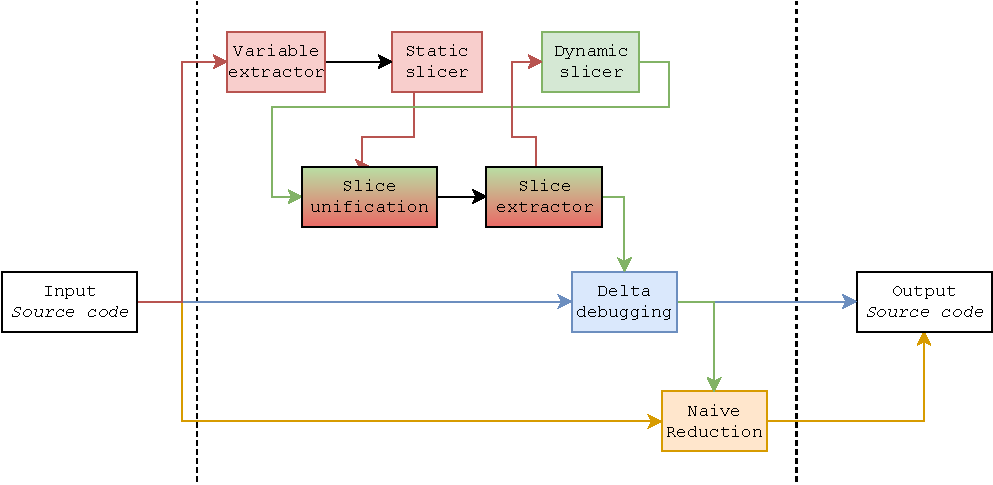
\includegraphics[scale=0.85]{components}
\caption{Communication between modules in three different pipelines:
Naive (orange), Delta (blue), Slicing (red and green).}
\label{img:components}
\end{figure}

Figure~\ref{img:components} shows a diagram of all available pipelines and 
their shared modules. 
Since some pipelines only add a preprocessing layer, they end up reusing 
the fundamental components of simpler pipelines.
Each module shown in the diagram will be described in the following sections.

\section{Shared components}\label{chap:components}

As was already mentioned, this project reuses several ideas and components 
in multiple approaches. 
One component does not necessarily translate to one idea. 
It often takes a couple of modules to capture that idea. 
The following subsections will describe each idea proposed in previous 
chapters. 
Each subsection will then outline components used by its particular idea.

\subsection*{Recursive visitor}

Some of the ideas in the following sections require us to traverse and alter 
the AST.
As explained in Section~\ref{chap:ast}, LibTooling allows us to traverse 
the AST using two methods. 
Splitting the code into code units could be done with either 
the \icode{RecursiveASTVisitor} or \icode{ASTMatchers}. 
We chose to implement the visitor interface to preserve more consistency 
across the project. 
Using a LibTooling visitor requires implementing three classes. 
Types of their implementation are described in detail in the following 
paragraphs.

\paragraph{Actions.} Each derivation of \icode{ASTFrontendAction} can have 
its own preprocessing and postprocessing steps.
Other than performing an action before and after a file is handled, it also 
creates a specific visitor.
In this project, we only utilize \icode{ASTFrontendAction} to create 
a consumer.
Moreover, the usage of actions tends to be module-specific. 
Usually, each component has its \emph{Actions.cpp} and \emph{Actions.h} files.
Further, some of the derivations use their custom factories.
By default, any \icode{ASTFrontendAction} can be created by calling 
the \icode{FrontendActionFactory::create()} method.
The method uses the default constructor and thus cannot provide any 
arguments for concrete \icode{ASTFrontendAction} implementations.
A workaround can be seen in \emph{Actions.cpp} files, most of which contain 
a custom factory.
The factory takes the necessary parameters, calls the desired constructor,
and passes them to a \icode{Consumer} instance in its \icode{create()} method.

\paragraph{Consumers.} This project distinguishes two types of 
\icode{Consumer} implementations. 
The first is a module-specific type. 
These \icode{Consumer} implementations contain high-level actions of 
a specific algorithm and are used for data transfer. 
For example, the \icode{VariantGeneratingConsumer} does not invoke any 
visitor instances. 
Instead, it keeps references to two more granular \icode{Consumer} objects. 
The \icode{VariantGeneratingConsumer} contains the main loop of the naive 
algorithm shown in Figure~\ref{chap:naive}. 
The pair of more granular consumers then carries out specific actions. 
The module-specific consumer also handles data exchanges between its more 
specific workers. 
One way of doing these exchanges is by keeping data structure instances 
inside the parent consumer. 
Another is by accessing the worker's internal states, either through their 
fields or getter methods. 
In summary, the module-specific consumer's job is to organize the granular 
parts of an algorithm, execute their actions, and collect their results.

The second \icode{Consumer} type is the shared consumer. 
These consumers are used for dispatching shared visitors, reporting their 
state, and collecting their data. 
The shared consumer responsible for code unit separation is 
the \icode{Dependency\-Mapping\-AST\-Consumer}. 
It dispatches a concrete visitor to the top-most node and offers getter 
methods to retrieve the visitor's data. 
This consumer also contains some logic in its 
\icode{HandleTranslationUnit} method. 
Other than dispatching the visitor, it also saves a visualization of 
the current AST. 
Other shared consumers might contain different logic in that method.


\paragraph{Visitors.} Visitors are once again separated into two types. 
A specific algorithm might use its unique visitor implementation to do 
an action such as slice extraction. 
This type of visitor is tied to a corresponding module-specific consumer. 
Similarly, shared visitors are also bound to their corresponding shared 
consumers. 
However, shared visitors are used for tasks that are used in both the naive 
and Delta algorithms. 
Those tasks are the node mapping and the variant generation. 
In our case, visitors contain the logic of a single iteration. 
Be it an iteration of the naive minimization or the Delta debugging; 
visitors are dispatched polynomially or even exponentially many times. 
The logic generally contains rules for handling each type of language 
construct. 
Two examples of such rules are:
\begin{itemize}
  \item Skipping the traversal of an implicit cast node of type 
  \icode{ImplicitCastExpr}, since removing it will not alter the source code.
  \item Creating a code unit for each statement that is not an expression.
\end{itemize}
The logic of a shared visitor is reused in multiple projects. 
This logic might include splitting the source code into code units. 
A module-specific visitor's logic is oriented to a particular problem, 
such as scanning the locations of statements in the code.

\subsection{Code units}\label{chap:codeunits}

Initially, a code unit was defined as any syntactically correct subset of 
the source code. 
It was then narrowed down to an atomic code unit - the smallest sensible 
syntactically correct source code element. 
Both the naive and the Delta algorithms use code units to perform their 
reductions. 
The goal is to split a given source code into partitions that can be later 
kept or removed. 
Those partitions would ideally not overlap and could be therefore 
independently removed.

We can split the input source code into code units by traversing its AST 
with a specified granularity. 
The idea is to analyze nodes based on hand-written rules. 
These rules specify which nodes are worth visiting and how to process them. 
While we are partitioning the source code, we might as well map the code's 
dependencies. 
This mapping can be done by extending our rules to perform specific lookup 
operations during the traversal. 
For example, the algorithm looks up all variable usages for a given variable 
declaration node. 
The results of those lookups are then kept in the dependency graph described 
in Section~\ref{chap:heuristics}.

\paragraph{Consumers.} The single consumer dedicated to code unit separation 
is implemented in the \icode{DependencyMappingASTConsumer} class. 
The consumer serves as a middle man for data transfers. 
Notably, it can retrieve data for the following structures:
\begin{itemize}
  \item Node mapping - this mapping is a lookup table that transitions 
  between a node's internal ID given by Clang and the current traversal 
  order number. 
  The traversal order number specifies the order in which the current node 
  is visited once the visitor is dispatched using 
  \icode{HandleTranslationUnit}. 
  The mapping is later transferred to other visitors to achieve the same 
  traversal order.
  \item Code units count - this property returns the total amount of code 
  units once their partitioning is complete.
  \item Dependency graph - is represented by a directional graph of nodes, 
  where each node is represented using its traversal order number. 
  Nodes in the graph might also contain additional information used for 
  debugging, such as their type and the code snippet they represent.
  \item Skipped nodes - this container serves as a list of nodes not worth 
  visiting. 
  These nodes might be too granular or solely implicit.
\end{itemize}
The consumer dispatches its concrete visitor, which carries most of 
the logic. 
The only standalone logic in the consumer is to dump a visualization of 
the source code based on the dependency graph.

\paragraph{Visitors.} What becomes a code unit is decided inside 
the \icode{MappingASTVisitor} class. 
The visitor traverses the AST in a postorder manner and stops at specified 
declarations, statements, and expressions. 
Each of these nodes must fulfill a predicate - their specific rule - to 
become a code unit. 
The node must not be a duplicate of an already visited node. 
It must also be a part of the main source file, i.e., not a part of a system 
header file. 
If the node satisfies all three requirements, it is considered a code unit. 
The node's ID mapping is then created, and the node is added to 
the dependency graph. 
On the other hand, if the node is not a valid code unit, it is added to 
the skipped nodes list. 
In that case, the next visitor will not consider visiting and manipulating 
the node when traversing the AST.

\subsection{Bitfield to variant transformation}\label{chap:variants}

Once the number of code units is known, we can create a bitfield of that 
size and generate representations of possible variants. 
The mechanism of generating bitfields was explained in 
Section~\ref{chap:naive}. 
This section describes the necessary parts of a technique that converts 
bitfields into source code variants. 
The idea is to flag AST nodes as code units and then traverse the AST again, 
removing the code unit nodes specified by a given bitfield. 
A single iteration of the variant-generating techniques produces one source 
code variant. 
The variant is created by starting with the original source code and 
gradually removing nodes. 
Each node has its index in the given bitfield. 
The index corresponds to the node's traversal order number. 
A node is removed if its corresponding bit is set to zero. 
To be more precise: the node is not removed from the AST. 
Instead, only its underlying source code is removed. 
The following paragraphs describe the code behind the removal.

\paragraph{Consumers.} All the necessary data for bitfield to source code 
conversion is acquired using the \icode{VariantPrintingASTConsumer}. 
This consumer dispatches its specific visitor and provides it with 
a bitfield. 
The visitor then removes snippets of the code based on that bitfield.
The consumer's job is to reset the visitor's state, launch it with 
the provided bitfield, and save its output into a specified file. 
The consumer can also access the visitor's internal state, namely its 
adjusted error line location. 
More details about this location can be found in the \emph{Visitors} section.

\paragraph{Visitors.} Similar to the code unit mapping issue, 
the \icode{Variant\-Printing\-AST\-Visitor} carries most of the conversion's 
logic.
It is provided with a bitfield, which it saves, and a \icode{Rewriter} 
instance, which it uses to generate the variant.
Section~\ref{chap:sts} describes the \icode{Rewriter} class in more detail.
Traversal of the source code is done in a postorder fashion to stay 
consistent with the previous visitor. 
The previous visitor shares its dependency graph and its list of skipped 
nodes.
This way, the \icode{VariantPrintingASTVisitor} can traverse the AST the way 
it was intended to. 

Each code unit, i.e., visited node, is removed if it fulfills specific 
requirements. 
First, the node's bit must be set to zero. 
Second, all its parent's bits must be set to one. 
The latter is a \icode{Rewriter} requirement. 
A parent node might represent a compound statement, and its children might 
be the individual statements inside the parent. 
If we were to remove the parent and one of its children, we would remove 
the same snippet twice. 
This catch would eventually lead to an error. 
The error can be avoided by only removing children while keeping their 
parents.

Removing code units tends to shift lines down. 
This phenomenon might lead to the statements on the original error line 
changing their location. 
The number of the error-inducing line must be adjusted. 
During the removal of each node, we extract its underlying code and analyze 
its presumed location. 
If the location comes before the original error-inducing line and 
the underlying code contains newline characters, we decrease 
the error-inducing line's number by the amount of found newline characters. 
At the end of the traversal, we are left with a correct line number for 
further validation, and all unwanted code units are removed. 
We are left with a \icode{Rewriter} instance whose buffer reflects 
the current variant. 
The visitor's iteration is done, and it is the consumer's job to save 
the contents of the buffer.

\subsection{Variant validation}\label{chap:validationimplementation}

Testing results on whether they are valid variants requires a standard 
interface, too.
Section~\ref{chap:verification} describes the steps in the process 
of validation.
The implementation contains three parts that are used in all approaches 
presented in this project.
Below is the description of compilation, analysis, and execution.

\paragraph{Compilation.} By calling the \icode{Compile} function in 
\emph{Helper.cpp}, one can invoke the Clang compiler driver.
The compiler has two goals.
Firstly, it filters out non-compilable and thus invalid variants.
Secondly, it prepares compilable variants for the execution stage.
The compilation can be invoked with a wide range of arguments.
In this case, it is provided with the \icode{-g} and \icode{-O0} options.
The former generates debug symbols for the executable, while the latter 
ensures reliable debugging by eliminating any compiler optimizations.
Compilation's output is printed to the standard output, and its exit status 
determines the function's return value.
If the compiler terminates with a valid exit code but does not create 
the binary, the function returns as if the compilation failed.
The binary is stored to a specified path, which by default is the same file 
path as the input source file.
The file extension is substituted with \icode{.exe}.

\paragraph{Static analysis.} Since our implementation is written in Clang's 
tooling library, we can reuse Clang's code and other Clang tools. 
Running the Clang Static Analyzer should not be a problem. 
However, we decided to skip the analysis step due to issues with processing 
the analyzer's results. 
Similarly to source code reduction, processing the analyzer's results would 
require us to understand the analyzer and write manual rules accordingly. 
Therefore, running the static analysis as a means of validation remains 
a proof-of-concept with no concrete implementation.

\paragraph{Execution.} Compiled binaries need to be validated at runtime.
This way, we check whether the program results in the desired runtime error.
Programs are executed in the LLDB environment.
LLDB provides Python API, which allows invoking more or less all of 
the debugger's commands.
The API is also available from C++ using a scripting bridge.
SWIG processes function calls made from C++.
They then produce bindings to the Python API.
Thanks to the scripting bridge, every validation step is written in C++.
The \icode{ValidateResults} function creates a debugging environment for every 
executable.

The programs are then run in separate processes.
During the execution, events are broadcasted from the forked processes.
The stack trace is investigated whenever the program broadcasts a stopped 
state, indicating a thrown exception.
If the symbol's location on top of the stack trace is the same as the one of 
the desired error, the program is tagged as valid.
Otherwise, the execution continues.

Previous sections, namely Chapter~\ref{chap:minimization}, have defined 
the \emph{location} of the error as a line and column number, as per 
Definition~\ref{def04:1}. 
Since Clang and LLDB are not necessarily precise with their source locations, 
we decided to relax the column requirement. 
Therefore, we only consider the error's line number. 
Additionally, we are required to check the error's description or its 
message. 
We do so by analyzing LLDB's stream and checking whether it contains 
the error message specified by the user.

\section{Naive reduction}\label{chap:naiveimplementation}

The algorithm for naive minimization is the foundation of this project. 
The approach and its heuristics were described in detail in 
Section~\ref{chap:naive}. 
The naive algorithm can guarantee minimality. Unfortunately, the same 
cannot be said for greedy approaches. 
Since this project focuses heavily on minimization, we dedicated 
a significant amount of time to improving the naive approach's 
implementation.

The reader has already seen most of this algorithm's implementation in 
Section~\ref{chap:components}. 
Nearly all shared components were created during the development of 
the naive approach. 
The implementation closely follows the algorithm shown in 
Figure~\ref{alg:naive}. 
As such, it required us to implement several vital mechanisms. 
First of all, the algorithm works with code units. 
As such, we had to create a way of splitting the code into several 
partitions. 
This lead to the implementation of a shared module that handles code units. 
That module has already been described in Section~\ref{chap:codeunits}. 
Second, we needed to convert bitfield representations into source code 
variants. 
This task required the development of a shared component that removes AST 
nodes based on a given bitfield. 
Details of this component can be found in Section~\ref{chap:variants}. 
The algorithm's last major requirement was the means to validate a variant. 
The implemented variant verification follows the steps described in 
Section~\ref{chap:verification}. 
Its implementation details as a shared module can be found in 
Section~\ref{chap:validationimplementation}.
The parts described above are not specific to the naive approach. 
Instead, they are used in the implementation of every suggested approach. 

However, the naive algorithm also uses its specific classes and functions. 
Two distinguishing factors are the bitfield manipulation and the validation 
of the dependency graph.

The naive algorithm works by iterating over all possible bitfield variants. 
Typically, the bitfield would be represented using an unsigned binary 
number. 
To~make working with the bitfield easier, we opted to represent it using 
a \icode{std::\-vector<\-bool>}. 
The vector is a good choice since its boolean variant uses 
a memory-efficient implementation in which each element only takes up 
a single bit. 
Working with the vector is also significantly more straightforward than 
with other representations. 
Possible bitfield variants are created by continuously incrementing 
the bitfield. 

However, the vector representation lacks the increment operation. 
We implemented it by flipping the first bit of the vector and keeping 
note of the carry-over bit. 
The implemented function's name is simply \icode{Increment}. 
As long as there is a carry-over bit, we keep flipping the consecutive 
indexes of the vector. 
Incrementing a bitfield where all bits are set to one leads to an overflow. 
While generating variants, we can prevent the overflow from happening by 
checking the \icode{IsFull} function. 
The function decides whether a given bitfield has all its bits set to one. 
The last used bitfield function is the \icode{IsValid} check. 
It determines whether a given bitfield might correspond to a valid source 
code variant. 

This function is also the first to utilize the dependency graph for its 
heuristic purposes. 
The function iterates over all bits in the bitfield. 
Each bit has to fulfill the following requirements. 
First, if the bit is set to zero, so must all of its children. 
This rule translates to ruling out both syntactically and semantically 
invalid variants. 
Second, if the bit represents a node in the criterion, i.e., 
the error-inducing location, it cannot be removed. 
This requirement preserves the failure-inducing line, ruling out pointless 
variants. 

The dependency graph validation is straightforward. 
Each node in the graph is represented using its traversal order number.
The exact number corresponds to the node's index in the bitfield. 
When validating all children of a particular node, we simply traverse 
a container of indices, checking whether the bitfield contains the desired 
bit value on each index.
The \icode{IsValid} function also calculates the size metric suggested in 
Section~\ref{chap:heuristics}. 
Each node has its presumed size in characters. 
The total size of the variant is calculated during the dependency graph 
validation. 
This way, we get an approximation of how large the source code variant is 
before generating it. 
The function returns a ratio of the size of the variant compared to 
the original size. 

This ratio serves two purposes. 
Firstly, the user can set their desired maximum ratio. 
If the user assumes the minimal variant is at most a quarter of 
the original size, they can set their target ratio to $0.25$. 
This assumption reduces the search space to only those variants whose 
presumed size is at most a quarter of the original size. 
Secondly, the implementation uses a sort of iterative deepening search. 
For a given number $k$, all valid bitfield variants are separated into $k$ 
bins. 
These bins represent parts of the interval from zero to the target ratio 
set by the user. 
The interval gets divided into $k$ evenly-sized parts, which then dictate 
the order in which the algorithm searches. 
First, the algorithm generates and validates all variants in the bin that 
contains the presumably smallest variants. 
If no valid result is found, the search continues with the bin containing 
the next smallest variants. 
Ideally, the search finishes faster than usual. 
This case would save time otherwise spent on generating all variants. 
In the worst case, the algorithm will generate and validate all possible 
variants, just like it did originally. 
Figure~\ref{alg:bins} shows the pseudocode of the bin heuristic.

\begin{figure}[h]
	\hrule height.8pt depth0pt \kern2pt
	\textbf{Input:} \\
	\hspace*{\algorithmicindent} $B \ldots$ a set of bins - containers of bitfield. \\
	\hspace*{\algorithmicindent} $L \ldots$ location of the error. \\
	\hspace*{\algorithmicindent} $A \ldots$ the input program's arguments. \\
	\textbf{Output:} The reduced source code. 
	\hrule height.8pt depth0pt \kern2pt
	\begin{algorithmic}[1]
		\ForAll{$Bin \in B$}
			\ForAll{$Variant \in B$}
				\If{IsValid($Variant$, $L$, $A$)}
					\Return $V$.
				\EndIf
			\EndFor
		\EndFor
	\end{algorithmic} 
	\hrule height.8pt depth0pt \kern2pt
	\caption{Binning search.} 
	\label{alg:bins}
\end{figure}

In the ideal world, we would know the exact size of a variant ahead of time. 
Knowing this, we could sort the variants before generating them, resulting 
in the best possible outcome. 
However, the presumed variant size is just an approximation. 
Clang's information on the underlying source code is not perfect. 
Using bins decreases the chances of classifying a non-minimal variant as 
the optimal result.

All the mentioned functions can be in the \emph{Common/\-src/\-Helper.cpp} 
file. 
The dependency graph resides in its file, 
\emph{Common/\-include/\-DependencyGraph.h}.

The mentioned functions are called from the algorithm's main loop. 
In our implementation, the loop is in the \icode{Handle\-Translation\-Unit} 
function of the \icode{Vari\-ant\-Generating\-Consumer} class. 
This consumer is specific to the naive reduction problem. 
It does not dispatch any visitors; it only governs two other consumer 
objects. 
Those objects are the instances of 
the \icode{Dependency\-Mapping\-AST\-Consumer} and 
the \icode{VariantPrintingASTConsumer} classes. 
The former partitions the input into code units, while the latter converts 
bitfields into source code variants. 
The body of \icode{HandleTranslationUnit} manages all data exchanges 
between the two consumers. 
It also contains the bitfield iteration logic. 
The consumer handles generating the variants, while their validation is 
invoked from the program's \icode{main} function. 

The consumer can be constructed using a custom factory. 
The \icode{Variant\-Generating\-Frontend\-Action\-Factory} function takes 
a reference to a \icode{GlobalCon\-text} object and later passes it to 
the visitor. 
The context is used for looking up the original input and the current state of the algorithm.

The problem-specific consumer can be found in 
the \emph{NaiveReduction/\-src/\-Consumers.cpp} file. 
The action that invokes the consumer is 
in \emph{NaiveReduction/\-src/\-Actions.cpp} and 
\emph{NaiveReduction/\-include/\-Actions.h}. 
The \icode{GlobalContext} resides in its own file under 
\emph{Common/\-include/\-Context.h}.

\section{Delta debugging}\label{chap:deltaimplementation}

Implementing the minimizing Delta debugging algorithm took significantly 
less time than expected. 
The implementation of the naive approach laid down a good enough foundation 
to make implementing Delta easy. 
The algorithm reuses existing components for code unit partitioning, 
bitfield to source code conversion, and validation. 
This section describes how it does so.

The minimizing Delta debugging algorithm is typically implemented using 
a text-modifying approach. 
The input test case could be split into $n$ partitions based on many factors.
One implementation might split the input on an exact number of characters, 
while another might do so on a specific number of lines. 
Text-oriented Delta debugging is not the only way of approaching Delta's 
implementation. 
Hierarchical Delta debugging (HDD) presented by Misherghi and 
Su~\citep{Misherghi06} handles the minimization using an AST. 
Implementing HDD would be ideal for this project since it we are working 
with the AST already. 
However, due to work already done on the naive approach in 
Section~\ref{chap:naiveimplementation}, we chose to implement a modified 
version of the minimizing Delta algorithm. 

Our implementation performs the following steps during each iteration:
\begin{enumerate}
  \item Input source code is partitioned into code units in the same manner 
  as in the naive approach, using the shared component described in 
  Section~\ref{chap:codeunits}.
  \item Bitfields are created in order to represent possible Delta 
  partitions and their complements. 
  The Delta algorithm splits the current test case into $n$ partitions and 
  their complements in each iteration. 
  This split translates to code units being assigned into specific variants. 
  Bitfields corresponds to one of 
  the $\alpha_1,\dots,\alpha_n,\beta_1,\dots,\beta_n$ variants. 
  The bitfield's elements are set to one if they represent snippets in their 
  variant.
  \item The bitfields are iterated over according to the algorithm in 
  Figure~\ref{alg:dd}. 
  Each bitfield is converted into source code using the component shown in 
  Section~\ref{chap:variants}. 
  The code is then validated. 
  If it causes the desired runtime error, it is regarded as the test case 
  for the next iteration. 
  The validation uses the module described in 
  Section~\ref{chap:validationimplementation}.
\end{enumerate}
The described approach is nearly equivalent to removing lines of the source 
code. 
However, it does leave some room for structure-based heuristics for future 
work.

The algorithm's main loop is inside the program's \icode{main} function. 
Each iteration invokes a custom visitor that handles it. 
Clang parses the current test case, and a \icode{Delta\-Debugging\-Consumer} 
instance performs its logic on the generated AST. 
The logic consists of the three steps shown in the previous paragraph: 
partitioning, generating variants, and validating. 
The iteration's result is then passed by reference back to the \icode{main} 
function. 

Similar to implementing the naive approach, the problem-specific consumer is 
invoked from a custom \icode{ASTFrontendAction}. 
The \icode{Delta\-Debugging\-Frontend\-Action\-Factory} function supplies 
data to the consumer. 
The data contains the following:
\begin{itemize}
  \item Iteration number - this number is used for correct file naming.
  \item Partition count - this number represents the number of even-sized 
  partitions into which the input should be split.
  \item Iteration result - the result is passed as a reference to 
  an \icode{enum}, which the consumer then specifies.
  \item Global context - analogically to the naive reduction's implementation, 
  the context serves to lookup information concerning the algorithm's input 
  and state.
\end{itemize}
The mentioned classes can be found in the following files: 
\begin{itemize}
  \item \emph{DeltaReduction/include/Consumers.h} 
  \item \emph{DeltaReduction/include/Actions.h} 
  \item \emph{DeltaReduction/src/Actions.cpp}
  \item \emph{Common/include/Context.h}
\end{itemize}

\section{External code}

As was already mentioned at the beginning of this chapter, implementing 
a slicer is out of this project's scope. 
We have turned to existing implementations of static and dynamic slicers. 
We know that these implementations will be more reliable and accurate. 
Below are the details concerning the two chosen slicer implementations. 
We were searching for LLVM-based slicers in the hope of running them natively 
during the reduction. 
However, due to compatibility reasons, the slicers cannot be easily shipped 
and executed with the current implementation of the rest of the project. 
Therefore, we run both slicers in their available Docker containers.

\paragraph{DG.} We chose DG as it is the best LLVM-based static slicer found. 
It slices LLVM bitcode and therefore requires the input in the compiled form. 
This requirement imposes the first obstacle - compiling the given source file 
to the LLVM intermediate representation. 
This task is not difficult for programs with a simple compilation command; 
however, handling large projects might be difficult. 
DG supports multiple criteria. 
One can slice w.r.t. either a function call or a variable on a given line. 
The variable criterion only works correctly for bitcode compiled with 
debugging symbols. 
DG also handles secondary slicing criteria, which are not required for this 
project. 

The output of DG is the sliced bitcode. 
The slice can be analyzed either by disassembling the bitcode or converting 
it to a list of line numbers using provided scripts. 
Nonetheless, we end up with a usable slice representation.

It should be noted that DG does not support C++ by design. 
Slicing its bitcode might not be an issue. 
However, there is a chance of encountering unsupported instruction.

DG is available on GitHub. 
The repository can be found at \url{https://github.com/mchalupa/dg}.

\paragraph{Giri.}

Giri is an LLVM-based backward dynamic slicer. 
The project started its development during the Google Summer of Code in 2013, 
and it has not received many updates since. 
It runs on a deprecated version of LLVM that cannot be installed on modern 
systems. 
In this project, we attempted to port Giri to a newer version of LLVM but 
ultimately failed. 
While most changes to Giri would have been trivial, others required much 
effort in reimplementing legacy constructs. 
Our update was therefore dropped.

One can use Giri via a \icode{Makefile}. 
This unconventional approach hides the standard interface of the slicer. 
Instead, the user specifies their desired criterion in a text file. 
Criteria must specify a path to the sliced source file and a line number. 
The text file is then passed to the \icode{make} command, and a prepared 
\icode{Makefile} is executed. 
The user can also specify a concrete instruction's number instead of its 
line number. 
However, this feature is not used in our project.

Similar to DG, Giri also produces a list of line numbers. 
This slice representation then has to be extracted from the original source 
code.
The dynamic slicer has a dodgy behavior when processing C++ code. 
Hence, we have decided to omit using the slicer in the slicing-based approach 
whenever an input written in C++ is present. 
We believe that in this case, Giri can be substituted by DG using argument 
injection.

Giri's repository can be found on GitHub on the following address: 
\url{https://github.com/liuml07/giri}.

\section{Systematic approach}

The systematic approach is a pipeline comprised of multiple steps. 
The steps are represented by components, some of which are shared with 
the previous implementation. 
The entire pipeline consists of a variable extraction tool, static and 
dynamic slicers, a slice unification tool, a slice extraction tool, 
the minimizing Delta debugging algorithm, and the naive approach. 
The motivation behind these steps and an overview of the algorithm can be 
found in Section~\ref{chap:systematic}.

This approach uses external code that cannot be trivially added to 
the project.
Therefore, it is launched and operated differently.
The external code forms two modules - containers. 
The static slicer is accessed via the DG container and the dynamic slicer 
via the Giri container. 
The unifying base is a Python script that invokes all necessary components.
The script uses Docker API to launch the DG container.
It also maps input and output directories to that container in order to send 
and retrieve data.
The container's launch command invokes the slicer to process the given input 
and store it in the given output directory.
The Giri container is launched analogically.

Both slicers produce a list of lines that represent the slices. 
The slicers are also run repeatedly, once for each variable on a given line. 
These variables are extracted using a \icode{VariableExtractor} tool. 
This module uses LibTooling's ASTMatchers to search for variable usages on 
a given line. 
The names of the symbols are then dumped into an output file. 
Slicers are executed with different criteria, and the criteria are taken 
from that file.
These runs generate multiple slices, which must be unified into a single one. 
The unification is simple. 
The slice is represented by a file containing a list of line numbers. 
The multiple generated files are merged, removing any duplicates. 
The result is a single file containing a single enhanced slice. 

This output needs to be processed further. 
The base script invokes the \icode{SliceExtractor} component. 
This module uses LibTooling's recursive AST visitor to access statements on 
given lines and preserve them. 
The program transforms a source file into the desired slice based on 
the given list of lines. 
First, the tool creates a container of preserved lines. 
Initially, the container consists of the lines given through the input. 
Later, the container expands by adding other previously poorly-mapped lines. 
For example, if a \icode{for} loop stretches over several lines and 
the slicer result only contains its first line, we must include those other 
lines as well. 
We do this by traversing the AST and inspecting nodes on given lines. 
If we encounter a node whose underlying code stretches over several lines, 
we include those lines in the container. 
The input source file is then opened and read, and the lines present in 
the container are preserved. 

Once the \icode{SliceExtractor} produces the desired source file, the file 
is considered the respective slicer's output.
This way, each step of the algorithm results in a valid source file.

Once the slicer preprocessing is done, the pipeline executes the implemented 
Delta debugging algorithm and finds a local minimum. 
The output is a source file which then serves as the input for the naive 
approach.
The Python script executes the naive algorithm, which then produces the 
desired results.
The implementation of both the naive reduction and the minimizing Delta 
debugging algorithm can be found in Section~\ref{chap:naiveimplementation} 
and Section~\ref{chap:deltaimplementation}, respectively.

The classes and functions used for implementing 
the \icode{VariableExtractor} and the \icode{SliceExtractor} modules can be 
found in their respective directories:
\begin{itemize}
  \item \emph{VariableExtractor/include}
  \item \emph{VariableExtractor/src}
  \item \emph{SliceExtractor/include}
  \item \emph{SliceExtractor/src}
\end{itemize}
The listed directories contain the problem-specific code. 
However, the tools also utilize code from shared components to carry out 
some repetitive tasks.
\chapter{Evaluation}



\chapter{Conclusion}

%% \addcontentsline{toc}{chapter}{Conclusion}

Source code minimization is a computationally demanding search problem. 
Generally, to achieve optimal results, i.e., the global minimum, one must 
generate and validate all possible results. 
Such a task results in exponentially many validations and is thus not feasible 
for any non-minor input. 
We attempt to avoid as many validations as possible, improving the running 
time while preserving the optimal result.

Approaches shown in this paper significantly differ in their time complexity. 
Analysis shows how a naive exponential algorithm can be sped up using 
heuristics. Those heuristics include iterative deepening and validating 
dependencies. 
A combination of search techniques and static analysis helps us formulate 
a more refined naive algorithm. 
Moreover, a rough approximation of the optimal result can be achieved 
in polynomial time by deploying a simple binary search technique. 
The approximation is denoted as a local minimum since it does not share 
the same optimality properties as the global minimum.

Relevant preprocessing techniques were presented, and their performance impact 
was measured. 
Running static and dynamic slicing reduced the source code's size 
significantly while preserving the desired runtime error. 
Furthermore, both slicers also conserved the cause of the error.
This paper shows that combining the mentioned preprocessing techniques with 
the presented algorithms yields good reduction results in average use cases. 
Such cases include unstructured, structured, and object-oriented source code. 
Unstructured programs saw the best results; we suppose that might be due to 
the nature of our implementation. 
The execution time is dramatically reduced compared to naive minimization. 
Introduced heuristics shaved off an immense number of validations in 
the average case. 
Though, the complexity for generating optimal results remains exponential in 
the worst case.

The premise of this project was to find a sophisticated way of minimizing 
a program while preserving the desired runtime error. 
We found out the slicing-based technique worked the best on all but trivial 
inputs. 
This result has confirmed and validated our beliefs held while formulating 
this technique.

\section{Future work}

Suggested techniques and algorithms have the potential to work well. 
They, however, require reliable and easy-to-use implementations. 
As mentioned in Section~\ref{chap:limitations}, our implementation of 
a minimization tool is not user-friendly due to several limitations. 
Upcoming enhancements focus on removing or relaxing these limitations. 
The main focus is on supporting a more comprehensive range of inputs. 
This goal can be achieved by implementing multi-file input support, reducing 
programs that interact with the user, and supporting multi-threaded 
applications.

Ideas that have been explained but not implemented are another focus of 
future attention. 
For example, the analysis explains how a static analyzer can be utilized to 
achieve better results. 
However, due to technical reasons, the implementation of this step could not 
be finished. 
There is room for more complicated heuristics, instrumentation, or pattern 
recognition for further improvements to speed and accuracy.

AutoPIE - the implementation of this project - can only be launched on 
Unix-based and Unix-like systems. 
We plan to extend the support to other platforms by creating a Docker image. 
This way, the implementation can be quickly shipped and executed. 
In order to improve the user interface, we plan on introducing an extension 
for Visual Studio Code, through which AutoPIE can be launched.

In the last months of working on this project, we came across CReduce - 
a tool for test case size reduction. 
Like our implementation, CReduce uses techniques such as Delta debugging to 
reduce the size of a program while preserving a wanted property. 
We might analyze CReduce in the future and perhaps contribute our findings 
to the project.


%%% Bibliography
%%% Bibliography (literature used as a source)
%%%
%%% We employ bibTeX to construct the bibliography. It processes
%%% citations in the text (e.g., the \cite{...} macro) and looks up
%%% relevant entries in the bibliography.bib file.
%%%
%%% The \bibliographystyle command selects, which style will be used
%%% for references from the text. The argument in curly brackets is
%%% the name of the corresponding style file (*.bst). Both styles
%%% mentioned in this template are included in LaTeX distributions.

% \bibliographystyle{plainnat}    %% Author (year)
\bibliographystyle{unsrt}     %% [number]

\renewcommand{\bibname}{Bibliography}

%%% Generate the bibliography. Beware that if you cited no works,
%%% the empty list will be omitted completely.

\bibliography{bibliography}

%%% If case you prefer to write the bibliography manually (without bibTeX),
%%% you can use the following. Please follow the ISO 690 standard and
%%% citation conventions of your field of research.

% \begin{thebibliography}{99}
%
% \bibitem{lamport94}
%   {\sc Lamport,} Leslie.
%   \emph{\LaTeX: A Document Preparation System}.
%   2nd edition.
%   Massachusetts: Addison Wesley, 1994.
%   ISBN 0-201-52983-1.
%
% \end{thebibliography}


%%% Figures used in the thesis (consider if this is needed)
\listoffigures

%%% Tables used in the thesis (consider if this is needed)
%%% In mathematical theses, it could be better to move the list of tables to the beginning of the thesis.
\listoftables

%%% Abbreviations used in the thesis, if any, including their explanation
%%% In mathematical theses, it could be better to move the list of abbreviations to the beginning of the thesis.
\chapwithtoc{List of Abbreviations}

%%% Attachments to the bachelor thesis, if any. Each attachment must be
%%% referred to at least once from the text of the thesis. Attachments
%%% are numbered.
%%%
%%% The printed version should preferably contain attachments, which can be
%%% read (additional tables and charts, supplementary text, examples of
%%% program output, etc.). The electronic version is more suited for attachments
%%% which will likely be used in an electronic form rather than read (program
%%% source code, data files, interactive charts, etc.). Electronic attachments
%%% should be uploaded to SIS and optionally also included in the thesis on a~CD/DVD.
%%% Allowed file formats are specified in provision of the rector no. 72/2017.
\appendix
\chapter{Attachments}

\section{Content of the attachment}
\dirtree{%
.1 Attachment{.zip}.
.2 AutoPie.
.3 Common \DTcomment{Source code shared by multiple projects.}.
.4 include.
.4 src.
.4 Makefile.
.3 DeltaReduction \DTcomment{Delta debugging algorithm's project directory.}.
.4 docs.
.4 include.
.4 src.
.4 Makefile.
.4 evaluate{.sh}.
.3 docs \DTcomment{Main documentation output path.}.
.3 EvaluationData \DTcomment{Evaluation dataset.}.
.3 NaiveReduction \DTcomment{Project directory of the naive approach.}.
.4 docs.
.4 include.
.4 src.
.4 Makefile.
.4 evaluate{.sh}.
.3 Scripts \DTcomment{Slicing-related components.}.
.4 SlicingReduction{.py} \DTcomment{Slicing-based minimization script.}.
.4 evaluate{.sh}.
.4 slice{.py}.
.4 unify{.py}.
.3 SliceExtractor \DTcomment{Slice-processing helper utility.}.
.4 docs.
.4 include.
.4 src.
.4 Makefile.
.3 VariableExtractor \DTcomment{Slice-preprocessing utility}.
.4 docs.
.4 src.
.4 Makefile.
.3 Makefile \DTcomment{Master Makefile that builds all components.}.
.3 buildLLVM{.sh} \DTcomment{Setup script for building LLVM.}.
}

The attachment is also available through an online repository. 
The repository can be found at \url{https://github.com/leskovde/AutoPIE}.

\section{User Documentation}

\subsection{System requirements}

The target system has to build AutoPIE, LLVM, Clang, and LLDB as well. 
Building the LLVM project utilizes a large number of system resources.  
In order to build the project correctly, the system must meet the following 
requirements:
\begin{itemize}
  \item The system must have at least 8 GB of memory.
  \item The system must have an x86-based CPU.
  \item The system should have at least 5 GB of free disk space and 
  optionally up to 40 GB of disk space for the debug build.
  \item The system must run a Linux distribution supported by LLVM 11.0.0.
\end{itemize}

Any mainstream Linux distributions released in the year 2020 and later are 
supported, provided they can run the tools specified in the following 
section. 
This list includes, for example, Manjaro 21.0, Arch Linux 2020.06.01, and 
Ubuntu 20.04.

\subsection{Prerequisites}

In order to build and launch AutoPIE, one must first install all underlying 
tools, libraries, and frameworks. 
The following list contains all tools and utilities that are required to 
build and run the project.

\begin{itemize}
  \item python2
  \item python3
  \item python-dev
  \item libedit-dev
  \item cmake
  \item ninja-build
  \item make
  \item gcc
  \item zlib
  \item coreutils
  \item graphviz
  \item docker
  \item docker-py
  \item swig
  \item doxygen
\end{itemize}

Additionally, the user must have the following packages available in their 
Python interpreter:

\begin{itemize}
  \item docker
  \item argparse
  \item shutil
  \item pathlib
\end{itemize}

Once these requirements are met, the user can proceed to build LLVM, Clang, 
and LLDB. 
The building process is lengthy, complex, and tedious. 
Therefore, we have created a script that automizes the process. 
The build can be launched by following the described steps.

\begin{enumerate}
  \item Navigate to the \icode{AutoPie} directory.
  \item Use \icode{chmod +x ./buildLLVM.sh} to give the script required 
  permissions.
  \item Run the script as root using \icode{sudo ./buildLLVM.sh}.
\end{enumerate}

The build script performs the following steps:

\begin{enumerate}
  \item It downloads the required version of the LLVM from the official 
  GitHub repository. 
  The specific version for this project is 11.0.0.
  \item It extracts the downloaded archive into a temporary directory.
  \item It creates a build subdirectory in the temporary path and navigates 
  to it.
  \item It executes the CMake command, which prepares the build 
  configuration for the required projects. 
  Notably, the Clang and LLVM projects are configured in x86 Release mode 
  with libraries and scripting support.
  \item It launches the Ninja tool, which builds the LLVM project. 
  It then installs the necessary headers and libraries into system paths.
  \item It exports the linker library path, which now contains 
  \icode{/usr/local/lib/}. 
  This export expires once the current shell is terminated.
\end{enumerate}

Confirm that the installation has finished correctly by checking the output 
of \icode{ls /usr/local/lib}. 
If the output contains libraries starting with \icode{libLLVM} and 
\icode{libclang}, the installation script has most likely performed all of 
its actions correctly. 
The linker now needs to know where to find the shared libraries. 
The user needs to ensure that the \icode{LD\_LIBRARY\_PATH} variable contains 
the path to \icode{/usr/local/lib}. 
In case it does not, the path can be added by executing the following command:

\icode{export LD\_LIBRARY\_PATH=\$LD\_LIBRARY\_PATH:/usr/local/lib/}.

If successful, the user can now use LLVM libraries when linking C++ projects.

\subsection{Building AutoPIE}

The project consists of several C++ binaries. 
These binaries can be built using makefiles in their respective directories. 
The \icode{AutoPie} directory also contains a \icode{Makefile} that builds 
all the projects. 
Once built, the binaries can be found in the following directories:
\icode{NaiveReduction} is available under 
\icode{AutoPie\-/NaiveReduction\-/build\-/bin\-/NaiveReduction}.
\icode{DeltaReduction} can be found under 
\icode{AutoPie\-/DeltaReduction\-/build\-/bin\-/DeltaReduction}.
The helper utilities \icode{VariableExtractor} and \icode{SliceExtractor} can 
be found in 
\icode{AutoPie\-/Vari\-ableExtractor\-/build\-/bin\-/VariableExtractor} 
and \icode{AutoPie\-/Slice\-Extract\-or/build\-/bin\-/Slice\-Extractor} 
respectivelly.

The slicing-based approach does not need to be built since it is implemented 
in Python. 
However, it utilizes all four mentioned C++ projects. 
Those must be present in order for the Python script to work correctly.

\subsection{Building documentation}

AutoPIE is extensively documented in its source code. 
We are aware of the fact that skimming through source code is not convenient 
for the user. 
Therefore we have created a Doxygen target for every \icode{Makefile} in 
the project. 
The user, with installed Doxygen, can build the documentation for individual 
components by navigating to their directories and using 
the \icode{make docs} command. 
The documentation is generated to the \icode{docs} directory in 
the component's subfolder as HTML or \LaTeX~files.

A more comprehensive way of using the generated documentation is by invoking
\icode{make docs} in the \icode{AutoPie} directory. 
This target generates the documentation of the entire project, include all 
of its components. 
The documentation is available in the \icode{AutoPie/docs} directory in both 
the HTML and \LaTeX~form.

It should be noted once again that the requirement for building 
the documentation is the Doxygen package.

\subsection{Running AutoPIE}

The user can execute the three approaches as follows:

\begin{itemize}
  \item The naive approach can be launched by executing 
  the \icode{NaiveReduction} program built from the earlier steps.
  \item The minimizing Delta debugging algorithm can be launched by 
  executing the \icode{DeltaReduction} program built from the earlier steps.
  \item The slicing-based approach can be launched by running 
  \icode{cd AutoPie\-/Scri\-pts\- \&\& python3 ./SlicingReduction.py}, 
  having built all other projects from the earlier steps.
\end{itemize}

Each project's required and supported arguments can be viewed using 
the \icode{--help} option available for each program and script.

The user can run the evaluation dataset by navigating to a subdirectory of 
an approach and launching \icode{evaluate.sh}. 

For example: \icode{cd autopie/NaiveReduction \&\& make \&\& ./evaluate.sh}.

When trying to run any component, the user might encounter an error while 
loading shared libraries. 
This error might stem from the fact that the installation script has not 
ended successfully, and therefore, \icode{/usr/local/lib} does not contain 
the necessary libraries. 
However, the more likely option is that the \icode{LD\_LIBRARY\_PATH} variable 
does not contain the proper path. 

The user can fix that by executing the following command:

\icode{export LD\_LIBRARY\_PATH=\$LD\_LIBRARY\_PATH:/usr/local/lib/}.

\openright
\end{document}
